\section{System Design}
\label{sec:fdsp-tpcelec-design}

%%%%%%%%%%%%%%%%%%%%%%%%%%%%%%%%%%%
\subsection{Grounding and Shielding}
\label{sec:fdsp-tpcelec-design-grounding}

\todo{Consider revising grounding section, which is copied directly from IDR}

In order to minimize system noise, the \dword{ce} cables for each \dword{apa} enter 
the cryostat through a single \dword{ce} flange, as shown in Figure~\ref{fig:connections}, creating, for grounding purposes, and integrated unit consisting of an \dword{apa} frame, \dword{femb} ground for all \num{20} \dword{ce} modules, TPC flange, and warm interface
electronics. To accomplish this,
the input amplifiers on the \dword{fe} \dwords{asic} have their ground terminals connected to the \dword{apa} frame. 
All power-return leads and cable shields are connected to both the ground plane of the \dword{femb} and to the TPC signal flange.

The only location where this integrated unit makes electrical contact with the 
cryostat, which defines \textit{detector ground}, is at a single point on the \dword{ce} \fdth board in the TPC signal flange where the 
cables exit the cryostat. Mechanical suspension of the \dwords{apa} is accomplished using insulated supports. 
To avoid structural ground loops, the \dword{apa} frames described in Chapter~\ref{ch:fdsp-apa} are 
insulated from each other.

Filtering circuits for the \dword{apa} wire-bias voltages are locally referenced to the ground plane of the \dwords{femb} through low-impedance electrical connections. This approach ensures a ground-return path in close proximity to the bias-voltage and signal paths. The close proximity of the current paths minimizes the size of potential loops to further suppress noise pickup.

Signals associated with the \dword{pds}, described in Chapter~\ref{ch:fdsp-pd}, are carried directly on shielded, 
twisted-pair cables to the signal \fdth. The cable shields are connected to the cryostat 
at the \dword{pd} flange shown in Figure~\ref{fig:connections}, and to the PCB shield layer on the \dwords{pd}. There is no electrical connection between the cable shields and the \dword{apa} frame.

%%%%%%%%%%%%%%%%%%%%%%%%%%%%%%%%%%%
\subsection{Distribution of Bias Voltages}
\label{sec:fdsp-tpcelec-design-bias}

\todo{Consider revising bias voltage section, which is copied directly from IDR (except for updated CR board figure)}

Each side of an \dword{apa} includes four wire layers as described in Section~\ref{sec:fdsp-apa-design}. 
%The innermost X-plane layer of wires is nominally biased at +820~V, with each wire AC coupled 
%to one of the 128 charge amplifier circuits on the \dword{femb}. The V-plane wire layer is effectively biased at zero volts, 
%with each wire directly connected to one of the charge amplifier circuits. The U-plane wire layer is nominally 
%biased at $-$370~V with each wire AC-coupled 
%to one of the 128 charge amplifier circuits. The outermost G-plane wire layer,
%which has no connection to the charge amplifier circuits, is biased at $-$665~V.
Electrons passing through the wire grid must drift unimpeded until they reach the $X$-plane 
collection layer. The nominal bias voltages are predicted to result in this electrically 
transparent configuration, and are given in Section~\ref{sec:fdsp-apa-design}. 

The filtering of wire bias voltages and AC coupling of wire signals passing
onto the charge amplifier circuits is done on capacitance-resistance (CR) boards that plug in between the \dword{apa} wire-board stacks and \dwords{femb}.
Each CR board includes single RC filters for the $X$- and $U$-plane wire bias voltages. In addition, each board has \num{48} 
pairs of bias resistors and AC coupling capacitors for $X$-plane wires, and \num{40} pairs for the $U$-plane wires. The coupling capacitors block DC while passing AC 
signals to the \dword{ce} motherboards.  A schematic diagram of the \dword{pdsp} \dword{apa} wire bias subsystem is illustrated in Figure~\ref{fig:CR-board}.

\begin{dunefigure}
[\dword{pdsp} \dword{apa} wire bias schematic diagram, including the CR board.]
{fig:CR-board}
{\dword{pdsp} \dword{apa} wire bias schematic diagram, including the CR board.}
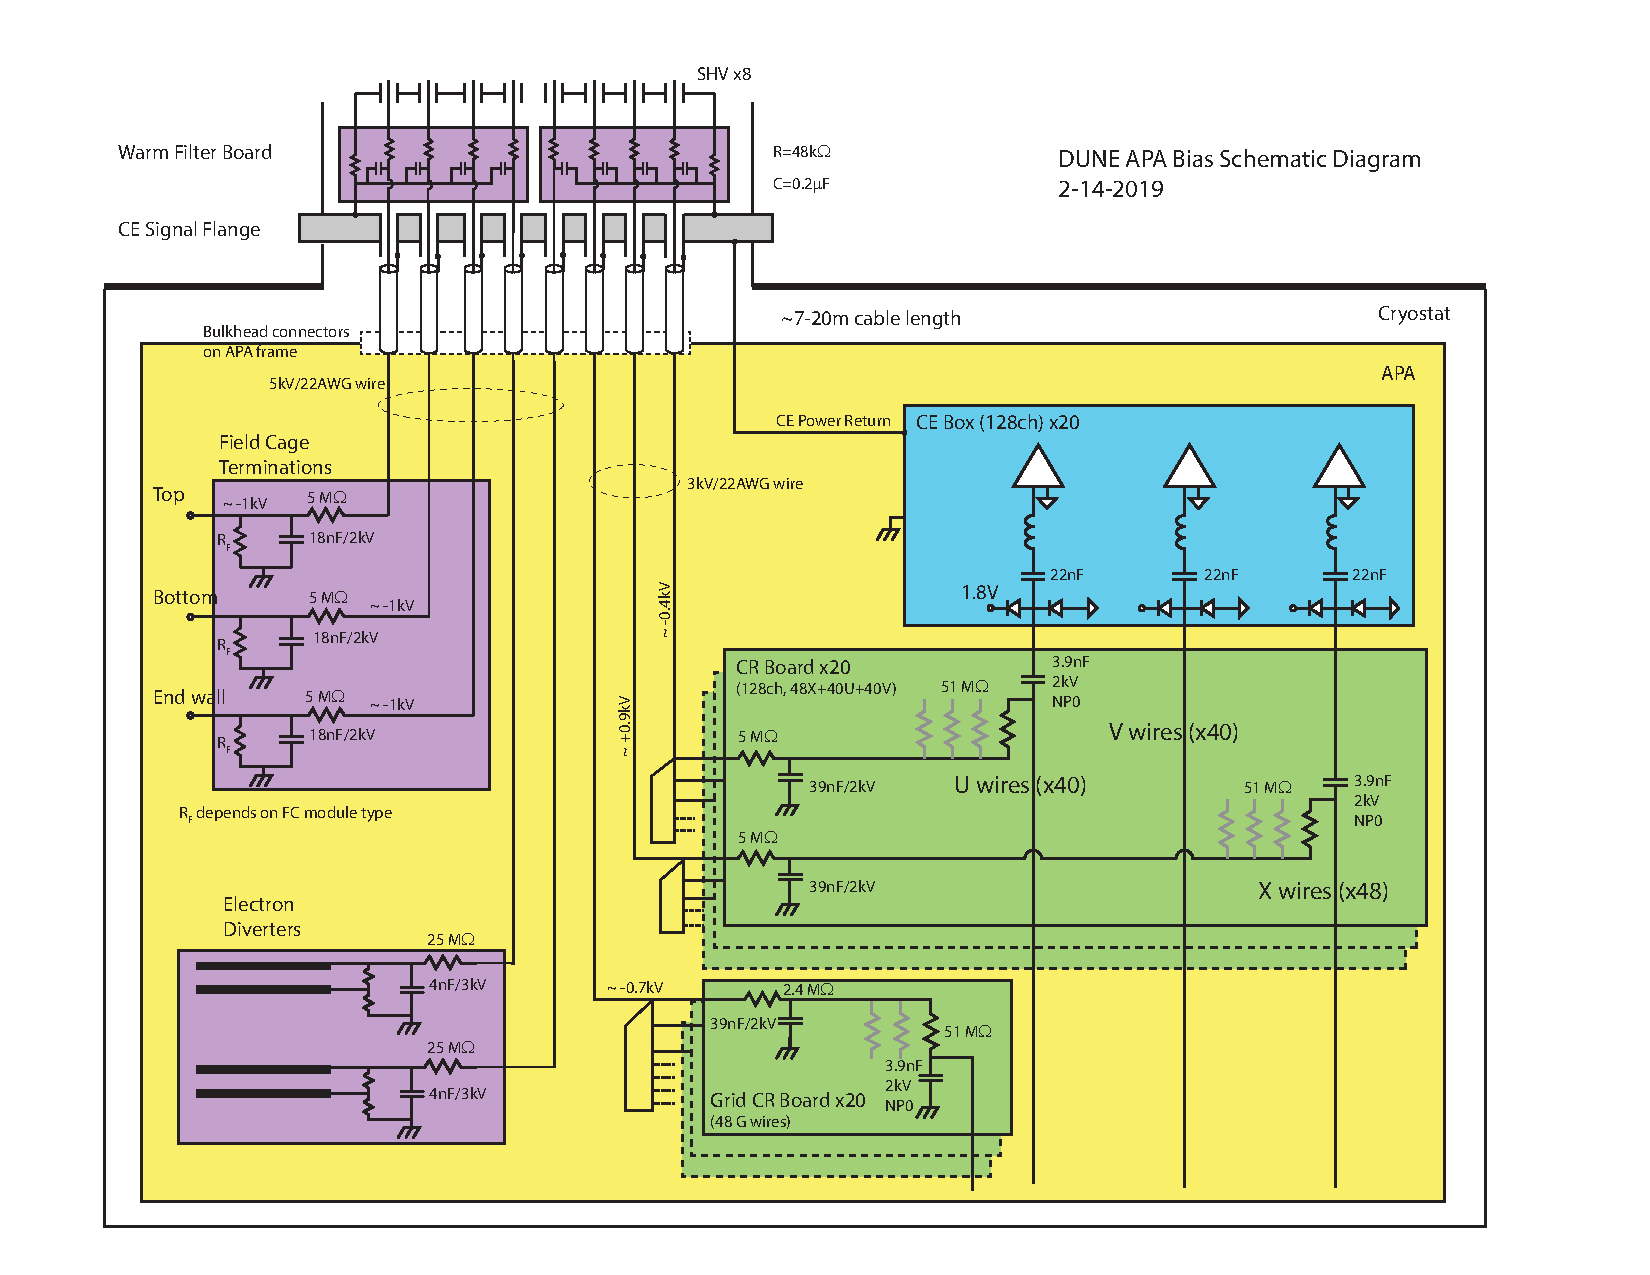
\includegraphics[width=0.8\linewidth]{sp-tpcelec-cr-board.pdf}
\end{dunefigure}

%Separate CR boards include a single R-C filter for the G-plane wires and 12 pairs of bias resistors and
%coupling capacitors.
%Groups of four wires are tied together to share single
%bias resistors and filter capacitors. These CR boards do not connect to the charge amplifier circuits on the \dword{femb}.

Clamping diodes limit the input voltage received at the amplifier circuits to between \SI{1.8}{V}\,$\pm$\,U$_D$, where U$_D$
is the breakdown voltage of the diode, $\sim$\SI{0.7}{V}.
The amplifier circuit has a \SI{22}{nF} coupling capacitor at input to avoid leakage current from the protection clamping diodes. 

%%% UNCLEAR, REMOVE FOR NOW
%Coupling capacitors for the X-plane and U-plane wires are required to block DC bias voltages.
%However they also impact the efficiency of the detector circuits.
%The sense wires are expected to have $\sim200$~pF of capacitance to the \dword{apa} frame.
%Induced or collected charges are effectively divided between the wire capacitance and the coupling capacitor.
%To achieve a charge-calibration accuracy of 0.5 percent or better,
%the coupling capacitors must be 4.7\,nF at ten percent tolerance, or 2.2\,nF at five percent tolerance.
%Voltage ratings should be at least 1.5 times the expected operating voltages.

Bias resistance values should be at least \SI{20}{\mega\ohm} to maintain negligible noise contributions.
The higher value helps to achieve a longer time constant for the high-pass coupling networks.
Time constants should be at least \num{25} times the electron drift time so that the undershoot in the digitized waveform
is small and easily correctable.
However, leakage currents can develop on PC boards that are exposed to high voltages over extended periods.
If the bias resistors are much greater than \SI{50}{\mega\ohm}, leakage currents may affect the bias voltages applied to the wires. The target value of \SI{50}{\mega\ohm} was used in \dword{pdsp}.

The bias-voltage filters are RC low-pass networks.
Resistance values should be much smaller than the bias resistances to control crosstalk between wires
and limit the voltage drop if any of the wires becomes shorted to the \dword{apa} frame.
The value of \SI{2.2}{\mega\ohm} was used in \dword{pdsp}.
Smaller values may be considered for %DUNE 
the \dword{spmod} although a larger filter capacitor would be required to maintain a given level of noise reduction.
The target value of \SI{47}{nF} was used in \dword{pdsp} for the filter capacitors.

%For the grid-plane bias filters, component values are less critical.
%If possible they will be identical to those used for the bias resistors and coupling capacitors
%(50~M$\Omega$ and 2.2 to 4.7\,nF).

%%%%%%%%%%%%%%%%%%%%%%%%%%%%%%%%%%%
\subsection{Front-End Motherboard}
\label{sec:fdsp-tpcelec-design-femb}

%%%%%%%%%%%%%%%%%%
\subsubsection{Overview}
\label{sec:fdsp-tpcelec-design-femb-overview}

Each \dword{apa} is instrumented with \num{20} \dwords{femb}.
The \dwords{femb} plug into the \dword{apa} CR boards, making the connections from the wires to the charge amplifier circuits as short as possible.
Each \dword{femb} receives signals from \num{40} $U$ wires, \num{40} $V$ wires, and \num{48} $X$ wires.
The baseline \dword{femb} design contains eight \num{16}-channel \dword{fe} (\dword{larasic}) \dwords{asic}, eight \num{16}-channel Cold \dword{adc} \dwords{asic}, and two \dword{coldata} control and communication \dwords{asic} (see Figure~\ref{fig:ce-scheme}).
The \dword{femb} also contains regulators that produce the voltages required by the \dwords{asic} and 
filter those voltages.
The \dword{larasic} inputs are protected by diodes and a series inductor.

\begin{dunefigure}
[The baseline \dword{ce} architecture.]
{fig:ce-scheme}
{The baseline \dword{ce} architecture. The basic unit is the \num{128}-channel \dword{femb}. Note that only one \dword{ce} flange is shown to simplify the illustration. Note that \dword{ssp} stands for \textit{SiPM Signal Processor} (see Chapter~\ref{ch:fdsp-pd}).}
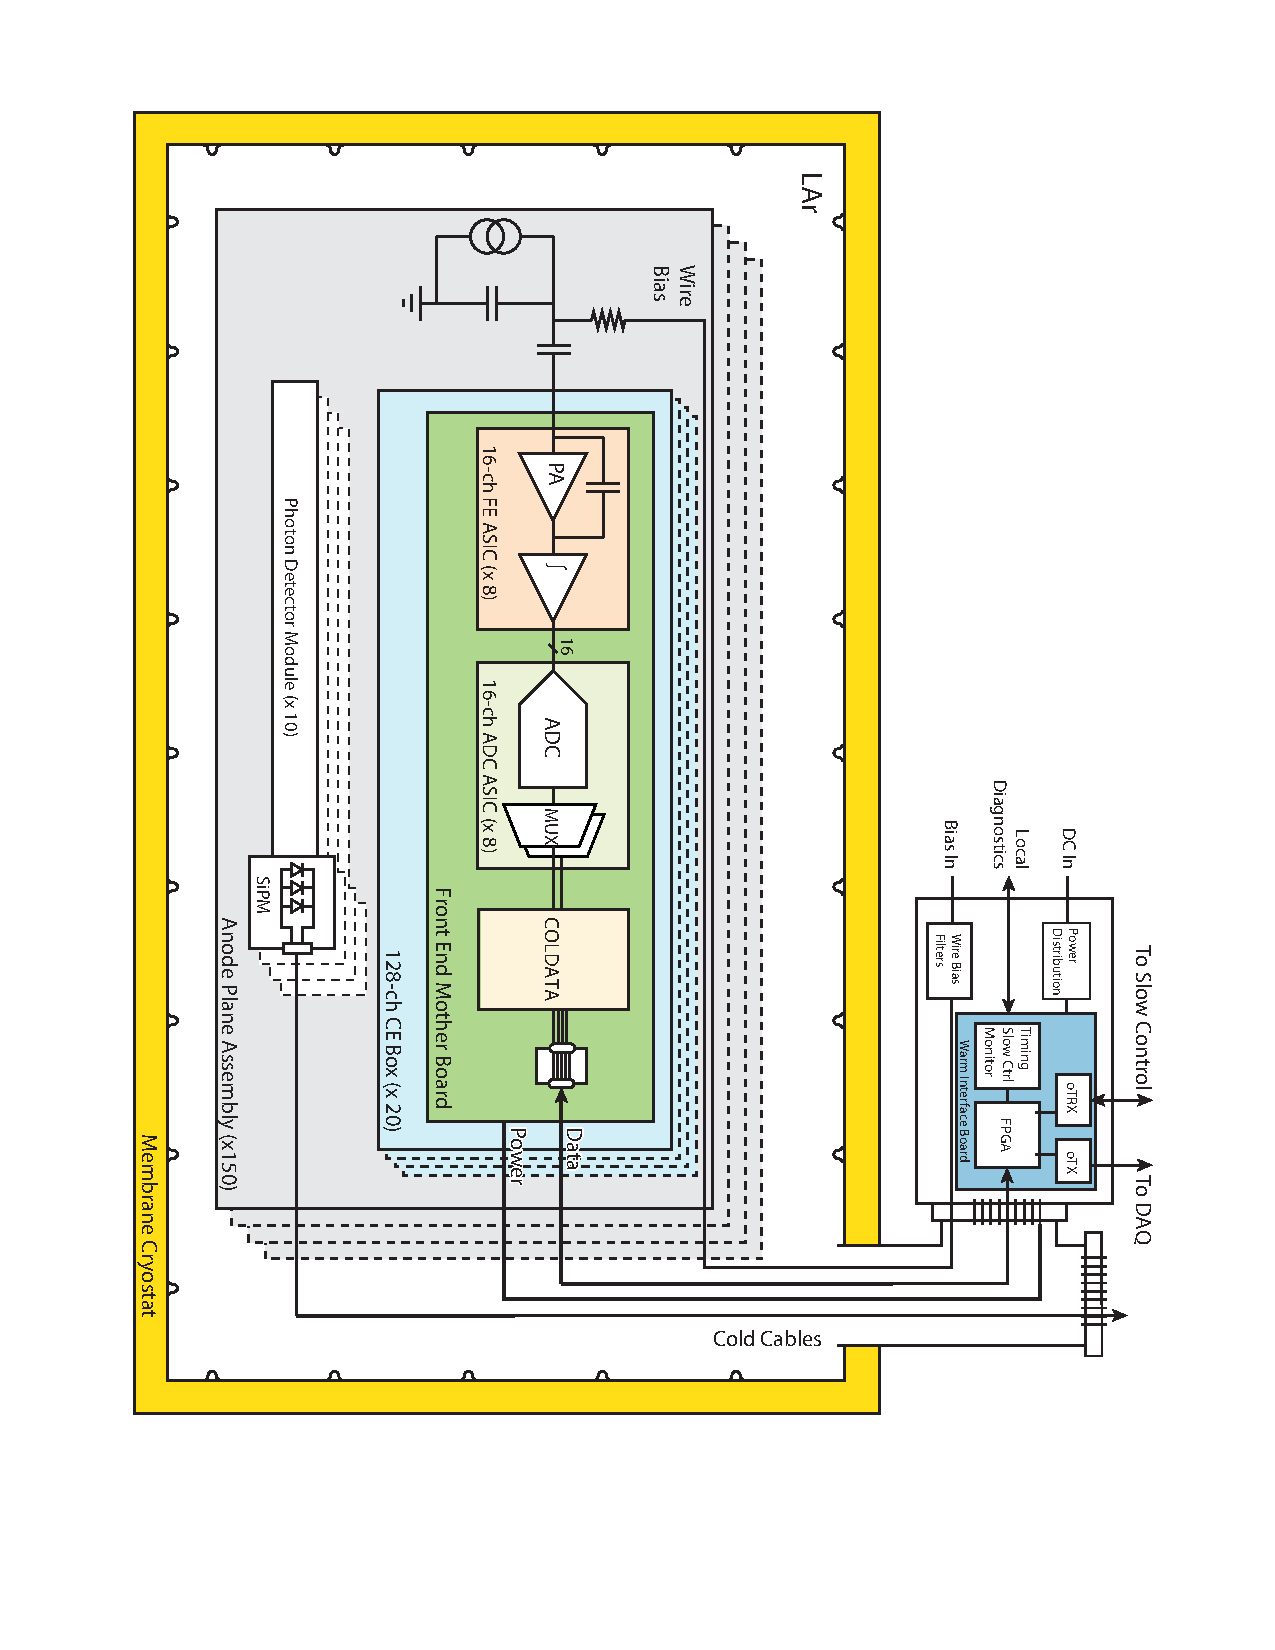
\includegraphics[width=0.9\linewidth,angle=90]{sp-tpcelec-schematic-v3.pdf}
\end{dunefigure}

The \dword{pdsp} version of the \dword{femb} (which uses a single \dword{fpga} on a mezzanine card instead of two \dword{coldata} \dwords{asic}) is shown in Figure~\ref{fig:femb}.

\begin{dunefigure}
[The complete \dword{femb} assembly as used in \dword{pdsp}.]
{fig:femb}
{The complete \dword{femb} assembly as used in the \dword{pdsp} detector. The cable shown is the high-speed data, clock, and control cable.}
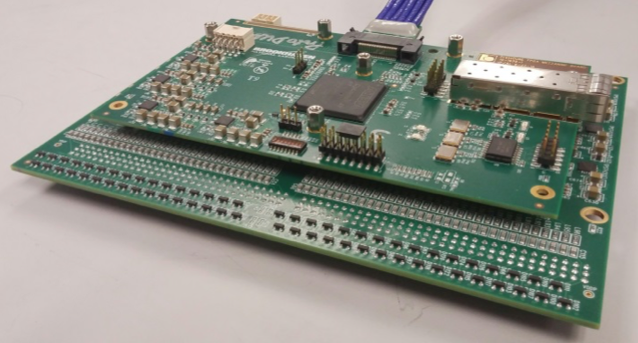
\includegraphics[width=0.6\linewidth]{sp-tpcelec-femb.png}
\end{dunefigure}

%%%%%%%%%%%%%%%%%%
\subsubsection{Front-End ASIC}
\label{sec:fdsp-tpcelec-design-femb-fe}

The analog front-end (FE) ASIC~\cite{DeGeronimo:2011zz} receives current signals from the TPC sense wires and provides a means to amplify and shape the signals for downstream signal digitization.  The FE ASIC has 16 channels, and is implemented using the TSMC 180nm CMOS process. It integrates a band-gap reference (BGR) to generate all the internal bias voltages and currents. This guarantees a high stability of the operating point over a wide range of temperatures, including cryogenic temperatures. The channel schematic of the FE ASIC is shown in Figure~\ref{fig:feasic1}. 

\begin{dunefigure}
[FE ASIC channel schematic]
{fig:feasic1}
{Channel schematic of FE ASIC, which includes a dual-stage charge amplifier and a 5$^{th}$ order semi-Gaussian shaper with complex conjugate poles. Circuits in red circles are programmable to allow different gain and peaking time settings.}
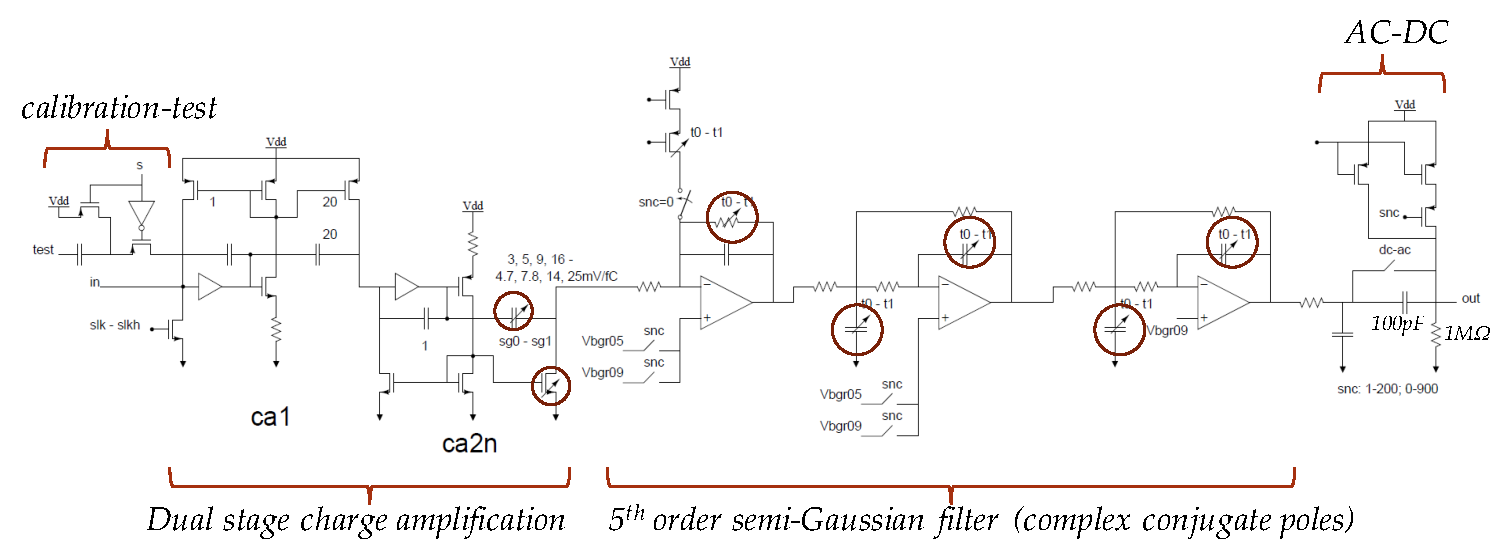
\includegraphics[width=0.99\linewidth]{sp-tpcelec-feasic-channelschematic.pdf}
\end{dunefigure}

Each FE ASIC channel has a dual-stage charge amplifier and a 5$^{th}$ order semi-Gaussian shaper as an anti-aliasing filter for the TPC signals. It has a programmable gain selectable from one of 4.7, 7.8, 14 or 25mV/fC (corresponding to full-scale charge of 300, 180, 100 and 55 fC), a programmable peaking time selectable from one of 0.5, 1, 2, and 3 $\mu$s, and a programmable baseline for operation with either the collection ($\sim$200mV) or the induction ($\sim$900mV) wires. Each channel has an option to enable the output monitor to probe the analog signal, and an option to enable a high-performance output driver that can be used to drive a long cable. 

Each FE ASIC channel has a built-in charge calibration capacitor which can be enabled or disabled through a dedicated register. The injection capacitance has been measured using a calibrated external capacitor. The measurements show that the calibration capacitance is extremely stable, changing from 184 fF at room temperature to 183 fF at 77 K. This result and the measured stability of the peaking time demonstrate the high stability of the passive components as a function of temperature. Channel-to-channel and chip-to-chip variation in the calibration capacitor are typically less than 1\%.

Shared among the 16 channels in the FE ASIC are the digital interface, programming registers, a temperature monitor and a bandgap reference monitor. It also has an option to enable AC coupling as mitigation of microphonics, a programmable bias current selectable from one of 0.1, 0.5, 1 or 5nA, and a programmable pulser generator with 6-bit DAC for calibration. 

The power dissipation of FE ASIC is about 5.5mW per channel at 1.8V supply voltage with output buffer disabled. The ASIC is packaged in a commercial, fully encapsulated plastic QFP 80 package. Figure~\ref{fig:feasic2} shows the response of FE ASIC for all gains and peaking times and both baselines. Note that the gain is independent of the peaking time; the same amount of charge produces the same peak voltage signal regardless of the peaking time.

\begin{dunefigure}
[FE ASIC response and layout]
{fig:feasic2}
{Response of FE ASIC for four gains, four peaking times, and both baseline values (left); layout of 16-channel FE ASIC version P3, where revisions with reference to version P2 are highlighted in yellow boxes (right).}
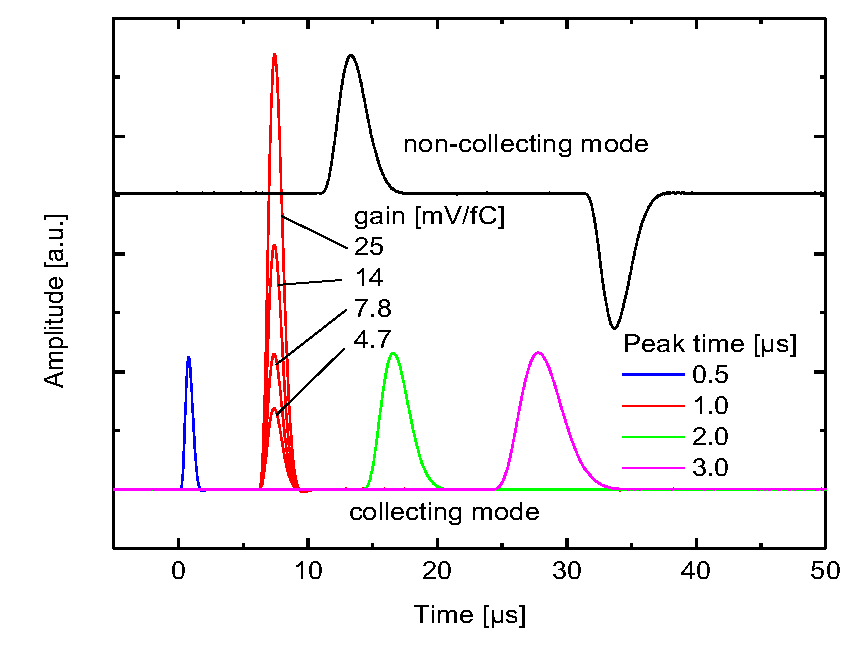
\includegraphics[width=0.48\linewidth]{sp-tpcelec-feasic-response.pdf}
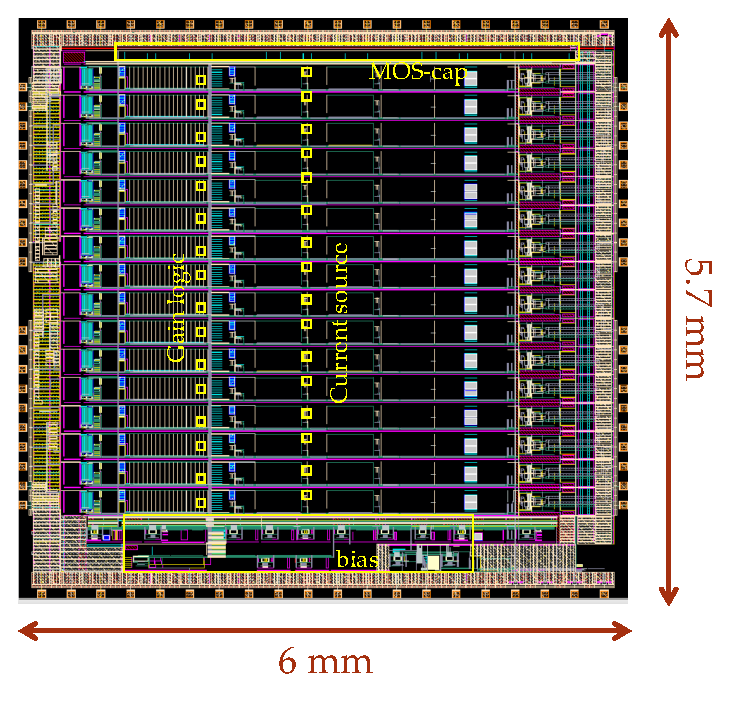
\includegraphics[width=0.48\linewidth]{sp-tpcelec-feasic-layout.pdf}
\end{dunefigure}

Prototype version P2 FE ASICs have been evaluated and characterized at room temperature and LN$_2$ (77 K) temperature. 960 P2 FE ASICs, total 15,360 channels, have been used to instrument six ProtoDUNE-SP APAs successfully. Due to exessive stress of package of FE ASIC in cryogenic temperature, FE channels have non-uniform baseline in collection mode, while the baseline DC voltage in induction mode is uniform. A new prototype version P3 has been fabricated in March 2018 to address this issue by making DC circuits for collection mode similar to the induction mode. At the same time, the default gain setting is changed to 14mV/fC. The layout of P3 FE ASIC is shown in \ref{fig:feasic2}, with modifications highlighted in yellow boxes. The P3 FE ASICs have been received and evaluated in September 2018, which shows both baseline in collection mode and default gain setting are working properly.

P3 FE ASIC will be further evaluated on FEMBs in various integration test stands for performance studies, including 40\% APA at BNL, ICEBERG TPC at Fermilab and APA7 at CERN. Test results of P3 FE ASIC will guide the development of next version P4 FE ASIC, which currently has a plan to implement single ended to differential (SE-DIFF) converter for interface to recently developed ADC ASIC. During the ProtoDUNE-SP operation, it was observed that the FE ASICs may enter into a saturation mode when large amount of charge ($>$ 50fC) is collected in the period of 10-50$\mu$s. This is being studied in the lab test stand, with the plan to address it in the P4 FE ASIC revision as well.

%%%%%%%%%%%%%%%%%%
\subsubsection{ADC ASIC}
\label{sec:fdsp-tpcelec-design-femb-adc}

COLDADC is a low-noise 12-bit ADC ASIC designed to digitize 16 input channels at a rate of 2 MHz.  COLDADC accepts either single-ended or differential inputs, and outputs digitized data to COLDATA.  COLDADC is implemented in TSMC 65 nm CMOS technology and has been designed by a team of engineers from LBL, BNL, and Fermilab.  The ASIC uses a conservative, industry standard design including digital calibration.  Each COLDADC receives 16 voltage outputs from a single LArASIC chip.  The voltages are buffered, multiplexed by 8 and input to two 15-stage pipelined ADCs operating at 16 MS/s.  The ADC uses the well-known pipelined architecture with redundancy\cite{PipelinedADC}\cite{CalibrationCorrection}.  Digital logic is used to correct non-linearity introduced by non-ideal amplifier gain and comparator thresholds in each pipeline stage, and an automatic calibration procedure is implemented to determine the constants used in this logic.  In order to maximize the probability that the first prototype COLDADC will perform well, the chip is highly programmable and many circuit blocks can be bypassed.  A block diagram of the chip is shown in Figure~\ref{fig:coldadc-blockdiagram}.  Each of the major blocks is described below.  COLDADC uses two bias voltages; 2.25V for I/O and 1.1V for the balance of the ASIC.

\begin{dunefigure}
[Baseline ADC ASIC block diagram]
{fig:coldadc-blockdiagram}
{Block diagram of baseline ADC ASIC (COLDADC) design.}
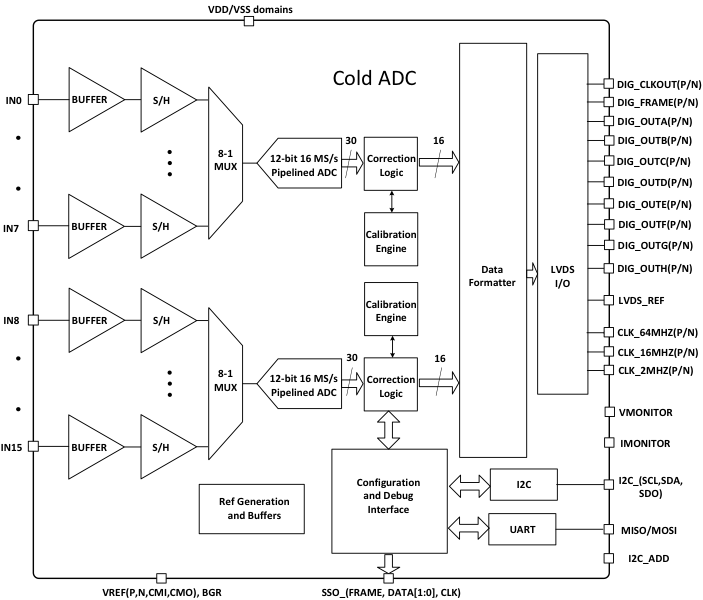
\includegraphics[width=0.8\linewidth]{sp-tpcelec-COLDADCblockdiagram.png}
\end{dunefigure}

\todo{Minor correction to figure needed: shows a non-existent 16 MHz clock}

All required reference voltages and currents are generated on-chip by programmable circuit blocks.  The most accurate reference voltage circuit is a band-gap reference based on a PNP (bipolar) transistor.  However, the TSMC 65 nm CMOS process does not allow the fabrication of high performance bipolar transistors, and bipolar transistors perform less well at liquid argon temperature than at room temperature.  Thus, a CMOS-based voltage reference has also been included in COLDADC.  In the event that both on-chip reference generation circuits fail, an external voltage reference can be used.

Many of the functional blocks in COLDADC are biased using current sources.  The bias points can be adjusted under digital control to trade power for performance and to allow different bias settings for different temperatures.  The input buffers, sample-and-hold amplifiers, ADC, and ADC reference buffers can independently be adjusted.  In addition, the band-gap reference circuit includes a bias current adjustment for an internal amplifier.

COLDADC has four possible ways to interface with LArASIC.  It can accept either single-ended inputs (provided by existing LArASIC chips) or differential inputs (foreseen for a future LArASIC upgrade).  In either case, to mitigate the risk that the input buffer circuits do not perform well, it is also possible to bypass the input buffers and apply the inputs directly to the sample-and-hold amplifiers.  The sample-and-hold amplifiers are separated into two groups of 8.  They sample the waveform at the rising edge of the (2 MHz) sampling clock.  An internally generated 16 MHz clock is then used to clock an 8-to-1 multiplexer which presents 8 samples in turn to one of the two ADC pipelines.

A block diagram of the COLDADC pipeline stages is shown in Figure~\ref{fig:coldadc-pipeline}.  Each of the 15 stages contains a low-resolution 1.5-bit analog-to-digital subconverter (ADSC) containing two comparators, a 1.5-bit digital-to-analog subconverter (DASC) that produces an voltage based on the two comparator outputs, an analog subtractor, a sample-and-hold amplifier (SHA), and a gain stage (with a gain of slightly less than two).  Each pipeline stage makes a three-level coarse decision based on the analog input voltage and then sends a voltage proportional to the quantization error resulting from the coarse decision to the next stage for further processing.  To limit power consumption, the stages of the ADC are scaled in area (and thus power) taking advantage of the fact that the accuracy requirements of the stages decline at each stage of the pipeline.

\begin{dunefigure}
[Pipeline circuit blocks in COLDADC ASIC]
{fig:coldadc-pipeline}
{Block diagram showing the circuit blocks in each pipeline stage of COLDADC.}
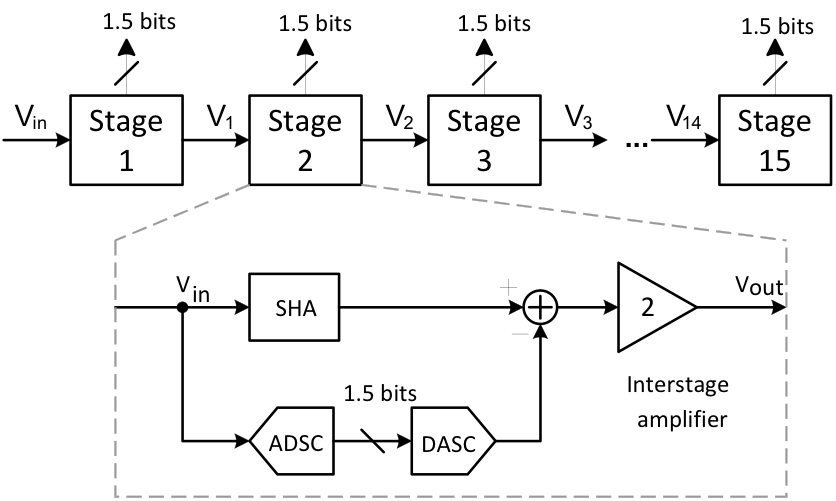
\includegraphics[width=0.8\linewidth]{sp-tpcelec-pipelinedADCstages.png}
\end{dunefigure}

\todo{Discuss correction/calibration logic and data formater}

The ten differential output drivers source and sink a current whose value can be digitally controlled.  The minimum current is 165 $\mu$A, which corresponds to approximately 3 mV peak-to-peak with 100$\Omega$ termination.  Seven additional levels spaced by 275 $\mu$A can be selected.  The maximum current is 2.07 mA, about 2/3 of the LVDS standard of 3.5 mA.

\todo{Discuss digital control}

%%%%%%%%%%%%%%%%%%
\subsubsection{COLDATA ASIC}
\label{sec:fdsp-tpcelec-design-femb-coldata}

The COLDATA ASIC was designed by engineers from Fermilab and Southern Methodist University.  It is responsible for all communications between the FEMBs and the electronics located outside the cryostat.  Each FEMB contains two COLDATA chips.  COLDATA receives command and control information from a Warm Interface Board (WIB).  Each COLDATA provides clocks to four COLDADCs and relays commands to four LArASIC front-end ASICs and four COLDADCs to set operating modes and initiate calibration procedures.  Each COLDATA receives data from four COLDADCs, merges the data streams, provides 8b/10b encoding, serializes the data, and transmits the data to the warm electronics over two 1.28 Gbps links.  These links are driven by line drivers with programmable pre-emphasis.  A block diagram of COLDATA is shown in Figure xx.yy.

Most commands are sent from a Warm Interface Board (WIB) to a FEMB using an I2C-like\cite{I2C} protocol.  However, while standard I2C uses single ended CMOS signals and a bidirectional data line, because of the long cables required between the warm interface electronics and the FEMBs, COLDATA uses low voltage differential pairs for both the I2C clock and data.  Point-to-point links are used and a separate link is used for data sent from warm to cold and for data sent from cold to warm.  In order to reduce the number of cables required, only one of the two COLDATA chips on an FEMB has its main I2C interface directly connected to a WIB.  That COLDATA chip relays I2C commands and data to the secondary COLDATA chip and relays I2C responses from the secondary COLDATA to the WIB.  Each COLDATA also relays I2C commands and data sent from the WIB to a COLDADC chip, as well as data sent back to the WIB from a COLDADC.  This link (on the FEMB) uses single ended CMOS signals, but data sent to the COLDADCs is still separate from data sent from the COLDADCs to the COLDATA.

COLDATA interprets commands intended for a LArASIC front-end chip and transmits them to the LArASICs using an SPI\cite{SPI} interface.  The configuration registers in LArASIC are configured to be loaded as a single shift register.  As data is shifted into LArASIC on the MOSI line, bits from the other end of the shift register are shifted out on the MISO line.  It is thus only possible to read LArASIC configuration registers while writing new configuration data.

COLDATA receives a master clock and a fast command signal from the WIB on a differential pair.  The master clock is nominally 64 MHz, but may be 62.5 MHz if that is preferred for reasons related to system synchronization.  It creates a 2 MHz ADC sampling clock by dividing the 64 MHz clock by 32.  Each COLDATA passes the 64 MHz clock and the 2 MHz clock to its four COLDADC chips.  If a 62.5 MHz master clock is used, then COLDADC will convert input data every 512 ns rather than every 500 ns.  The fast command line is used for signals that must be executed at a known time.

Both COLDATA and COLDADC are implemented in the TSMC 65nm CMOS process.\cite{TSMC65} The designs were done using cold transistor models produced by Logix Consulting.\cite{Logix} Logix made measurements of Fermilab-supplied TSMC 65 nm transistors at LN2 temperature and extracted and provided to Fermilab SPICE \cite{SPICE} models models valid at LN2 temperature.  These models were used in analog simulations of COLDATA and COLDADC subcircuits.  In order to eliminate the risk of accelerated aging due to the hot carrier effect,\cite{Hot-electron} no transistor with channel length less than 90 nm was used in either ASIC design.  A special library of standard cells using 90 nm channel length transistors was developed by members of the University of Pennsylvania and Fermilab groups.  Timing parameters were developed for this standard cell library using the Cadence Liberate tool\cite{Liberate} and the Logix SPICE models.  With the exception of the COLDATA PLL, serializer, and output driver, the digital sections of COLDATA and COLDADC were synthesized from Verilog code using this standard cell library and the Cadence Innovus tool.\cite{Innovus} Innovus was also used for the layout of the synthesized logic.

\todo{Include description of Fast Command interface, include performance examples (1.28 Gbps link over 25m of warm Samtec cable), include possible upgrade paths}

%%%%%%%%%%%%%%%%%%
\subsubsection{Alternative Designs}
\label{sec:fdsp-tpcelec-design-femb-alt}

%%%%%%%%%
\subsubsubsection{CRYO Option}
\label{sec:fdsp-tpcelec-design-femb-alt-cryo}

The SLAC CRYO \dword{asic} differs from the baseline three-chip design in that it combines the functions of an analog preamplifier, \dword{adc}, and data serialization and transmission for \num{64}~wire channels, into a single chip.
It is based on a design developed for the nEXO experiment\footnote{Enriched Xenon Observatory, \url{https://www-project.slac.stanford.edu/exo/about.html}.} and differs from it only in the design of the preamplifier, which is modified to account for the higher capacitance of the DUNE \dword{spmod} wires compared to the small pads of nEXO.
The \dwords{femb} constructed using this chip would use only two \dwords{asic}, compared to the \num{18} (eight~FE, eight~\dword{adc} and two~COLDATA) needed in the baseline design.
This drastic reduction in part count may significantly improve \dword{femb} reliablity, reduce power, and reduce costs related to production and testing. 

Figure~\ref{fig:cryo-architecture} shows the overall architecture of the CRYO \dword{asic}, which will be implemented in \SI{130}{nm} \dword{cmos}.
It comprises two identical, \num{32}-channel blocks. 
The current signal from each wire is amplified using a preamplifier with pole zero cancellation and an anti-alias fifth-order Bessel filter applied. 
Provisions are also made for injection of test pulses. 
Gain and peaking time are adjustable to values similar to those of the baseline design.

\begin{dunefigure}
[Overall architecture of the CRYO \dword{asic}.]
{fig:cryo-architecture}
{Overall architecture of the CRYO \dword{asic}.}
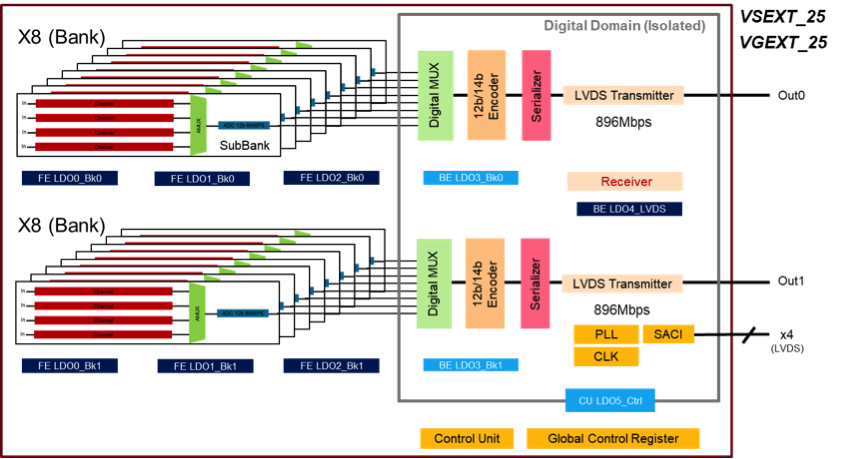
\includegraphics[width=0.8\textwidth]{sp-tpcelec-cryo-schematic.png}
\end{dunefigure}

The \dword{adc} uses \SI{8}{MHz} successive approximation registration (SAR), so that four input channels are multiplexed onto a single \dword{adc}. The data serialization and transmission block employs a custom 12b/14b encoder, so that \num{32} channels of \num{12}-bit, \SI{2}{MHz} data can be transmitted with a digital bandwidth of only \SI{896}{Mbps}, which is significantly less than the required bandwidth of the baseline, which is \SI{1.28}{Gbps}.

One key concern with mixed signal \dwords{asic} is the possibility of interference from the digital side causing noise on the very sensitive preamplifier. 
Fortunately, there are well established techniques for substrate isolation described in the literature~\cite{yeh}, which have been successfully employed in previous \dwords{asic} produced by the SLAC group.% Figure \ref{fig:cryo-substrate} shows how substrate isolation is achieved. 

%\begin{dunefigure}
%[Depiction of the substrate isolation technique that allows combining analog and digital circuitry on the same CRYO \dword{asic}.]
%{fig:cryo-substrate}
%{Depiction of the substrate isolation technique that allows combining analog and digital circuitry on the same CRYO \dword{asic}.}
%\includegraphics[width=0.6\textwidth]{tpcelec-cryo_substrate.png}
%\end{dunefigure}

The infrastructure requirements for a CYRO \dword{asic}-based system are similar to those of the baseline option. However, in most cases, somewhat fewer resources are needed:
\begin{itemize}
\item{A single voltage is needed for the power supply. This is used to generate two supply voltages using internal voltage regulators.}
\item{The output digital bandwidth on each of the four lines in an \dword{femb} is \SI{896}{Mbps}. This is lower than the baseline option due to the custom 12b/14b encoder of the CRYO chip. }
\item{The warm interface is different. Only a single clock is needed (\SI{56}{MHz}) and the configuration protocol is the SLAC \dword{asic} Control Interface (SACI)~\cite{SACI} rather than I2C.}
\end{itemize}

The first iteration of the CRYO \dword{asic} design was submitted for fabrication to MOSIS in November 2018.  The first protoypes are expected to be received in January, 2019. Simulation-based studies have already been performed; at \SI{0.8}{\micro\second} peaking time and an input capacitance of \SI{200}{pF} (similar to that expected in the DUNE \dword{spmod}), the \dword{enc} is approximately \num{500}\,e$^-$.  This noise level is similar to that expected with the baseline \dword{fe} and \dword{adc} \dword{asic} design in \lar with the same input capacitance.  Submission to the \dword{asic} foundry is imminent and the first prototypes should be received by summer 2018. They will first be tested in an existing test stand at SLAC. Subsequent tests are planned for a small test TPC at \fnal and on an \dword{apa} in the \dword{pdsp} cold box; these test facilities are described in Section~\ref{sec:fdsp-tpcelec-qa-facilities}.

In January 2019, stand-alone tests of the CRYO \dword{asic} will begin. In addition to standard ``bringing-up'' tests, measurements of noise (Equivalent Noise Charge), linearity (Equivalent Number of Bits) and bit-error rate will be performed. Figure~\ref{fig:cryo-results} shows ``place-holder'' plots of the type that will be produced in the initial stand-alone tests.

\begin{dunefigure}
[Results of stand-alone tests of the CRYO \dword{asic}.]
{fig:cryo-results}
{Results of stand-alone tests of the CRYO \dword{asic}. Top row shows Equivalent Noise Charge measured in each channel at room temperature (left) and Liquid Nitrogen Temperature (right). Bottom row shows the Equivalent Number of Bits (ENOB). }
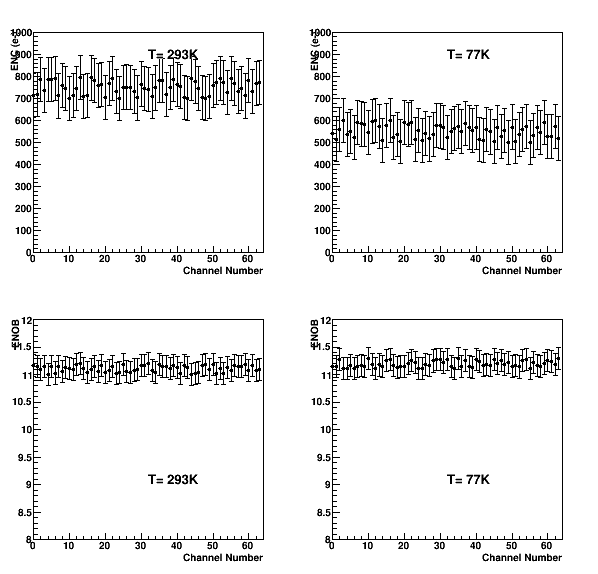
\includegraphics[width=0.8\textwidth]{sp-tpcelec-cryo-results.png}
\end{dunefigure}

%%%%%%%%%
\subsubsubsection{COTS ADC Option}
\label{sec:fdsp-tpcelec-design-femb-alt-cots}

The SBND collaboration has been exploring the COTS (``Commercial Off The Shelf'') ADC option for the TPC readout electronics development since Spring 2017~\cite{Chen:2018zic}. Market survey was carried out, few candidate ADCs in SAR architecture were identified with 100\% cold yield. Since July 2017, a lifetime study plan was developed to evaluate COTS ADC in two different phases, exploratory phase and validation phase. The lifetime study was focused on the ADI AD7274 implemented in TSMC 350nm CMOS technology given the optimum performance in cryogenic operation compared to other candidates.

During the exploratory phase, fresh samples of COTS ADC AD7274 were stressed with higher than nominal operation voltage, such as 5 V, while power consumption (current drawn) was monitored continuously. Periodically the sample would be operated at nominal voltage (V$_{DD}$ = 2.5V and V$_{REF}$ = 1.8V) for performance characterization test, where both DNL (Differential Non-Linearity) and INL (Integral Non-Linearity) were monitored and analyzed in addition to the current monitoring. Stress test results were used to extrapolate the lifetime of the COTS ADC. It was determined that the current drop of 1\% on the V$_{DD}$ is used as degradation criteria for lifetime study. In the validation phase, more devices have been tested following the criteria developed, to collect more data to validate what was learned in the exploratory phase.

The lifetime projection of COTS ADC AD7274 from the stress test with V$_{DD} >$ 5V is shown in Figure~\ref{fig:cotsadc-lifetime}. With ADC7274 operated at 2.5V which is less than the nominal 3.6V for 350nm CMOS technology, the projected lifetime is more than than 10$^6$ years.

\begin{dunefigure}
[Lifetime projection of COTS ADC]
{fig:cotsadc-lifetime}
{Lifetime projection of COTS ADC AD7274 from the stress test with V$_{DD} >$ 5V. The current drop of 1\% on the V$_{DD}$ is used as degradation criteria. With nominal operation voltage of 3.6V for 350nm CMOS technology, the lifetime is projected more than 100 years. For SBND and DUNE far detector, the AD7274 will be operated at 2.5V to gain further margin, the expected lifetime is more than 10$^6$ years.}
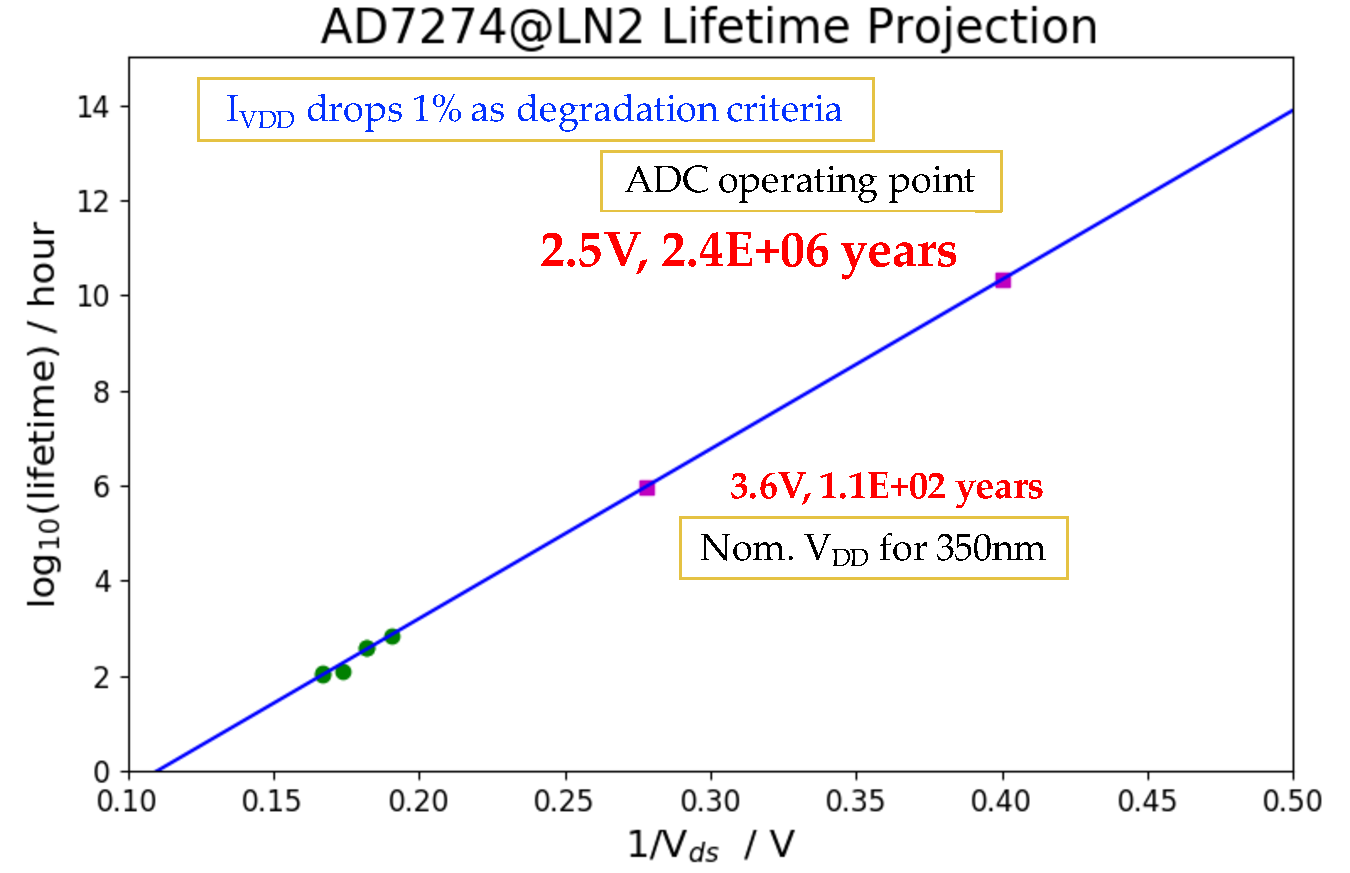
\includegraphics[width=0.8\linewidth]{sp-tpcelec-cotsadc-lifetime.pdf}
\end{dunefigure}

Based on the lifetime study of AD7274, an FEMB with COTS ADC has been developed and characterized for SBND experiment. The integration test was carried out with 40\% APA at BNL and showed satisfactory noise performance in Figure~\ref{fig:cotsadc-fembenc}. The COTS ADC AD7274 serves as a backup solution for DUNE far detector TPC readout electronics system. The current plan is to evaluate it in the small TPC ICEBERG at Fermilab. Ten FEMBs with COTS ADC are being produced and will be used to instrument ICEBERG TPC for system integration test in early 2019. 

\begin{dunefigure}
[ENC measurement of FEMB with COTS ADC]
{fig:cotsadc-fembenc}
{The ENC measurement of FEMB with COTS ADC mounted on 40\% APA at BNL. The picture of FEMB is shown in the top left corner. The induction plane (4 m wire) has ENC $\sim$ 400$e^-$ with 1$\mu$s peaking time, and the collection plane (2.8 m wire) has ENC $\sim$ 330$e^-$ with 1$\mu$s peaking time.}
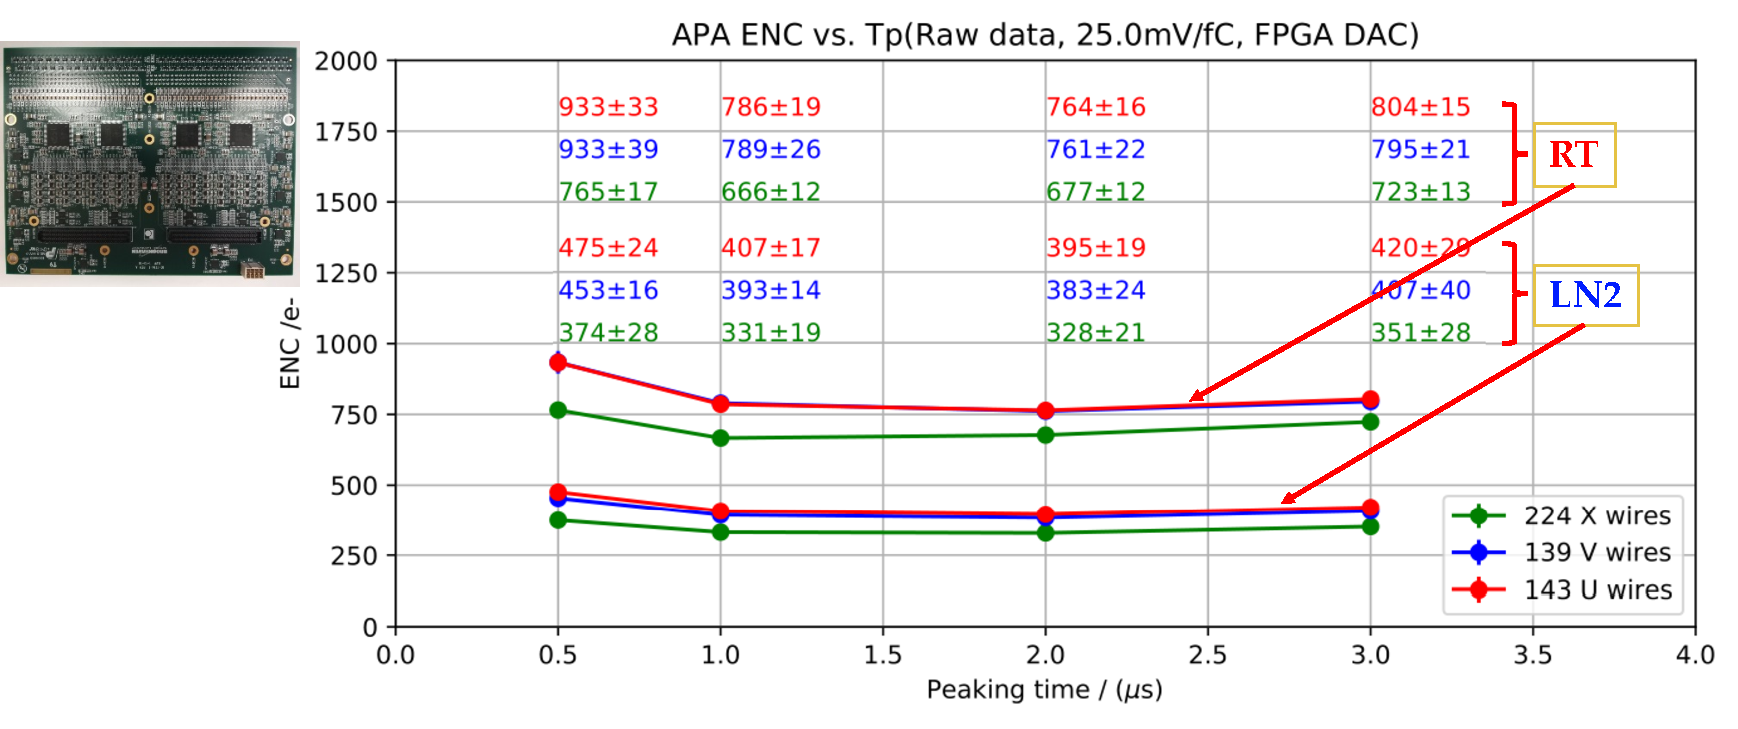
\includegraphics[width=0.99\linewidth]{sp-tpcelec-cotsadc-fembenc.pdf}
\end{dunefigure}

%%%%%%%%%%%%%%%%%%
\subsubsection{Procedure and Timeline for ASIC Selection}
\label{sec:fdsp-tpcelec-design-femb-selection}

We are currently pursuing two different \dword{asic} designs
and we are also planning on qualifying the commercial off the
shelf ADC solution that will be used for the SBND experiment.
For the moment we are planning to continue the development of
both the three \dword{asic} solution and of the CRYO \dword{asic}
for at least a second iteration before taking a decision on
the \dword{asic} solution to be used for the construction of
the DUNE \dword{sp} detector. This assumes that the \dwords{femb}
populated with the first set of prototypes of the two kinds of
\dwords{asic}, expected to become available in Spring 2019,
demonstrate a performance at least similar to that of the
boards used for the \dword{pdsp} detector. We plan to have a
review in Fall 2019 to review the results of system tests
discussed in Section~\ref{sec:fdsp-tpcelec-qa}. We will also
review results from measaurements of the components' lifetimes,
discussed in Section~\ref{sec:fdsp-tpcelec-qa-reliability}. In this review
we will also decide whether there are any changes on the list
of requirements for the \dwords{asic} and the further development
plans for the two solutions. We expect that the following iteration
of the design, fabrication, and testing of the \dwords{asic} and
\dwords{femb} will take an additional twelve months. At
the end of this process, when results from standalone tests of the
\dwords{asic} and system tests of the \dwords{femb} will become
available, we should be in the position of deciding which \dword{asic}
solution to adopt for the construction of DUNE \dword{sp} detector.

We have not yet defined the exact criteria to be used for the
\dword{asic} selection. Performance in system tests will obviously
be one of the driving criteria, but we will need to pay attention
also to reliability issues (which could favor the single \dword{asic}
solution, that requires \dwords{femb} with fewer connections), to
power density (which could be less favorable for the CRYO solution),
and to the costs and resources required during the construction
and testing of \dwords{femb}. We are planning to charge a committee
to draft a series of recommendations on how to perform the
\dword{asic} selection such that they can be reviewed in the Fall
of 2019, prior to the decision on the second cycle of design for
\dwords{asic} and \dwords{femb}. Once the second cycle of design
and testing is complete these recommendations will be used by the
committee charged with the final design review to suggest a
preferred option for the \dword{asic} solution to be used for the
construction of DUNE \dword{sp} detector. The recommendation of
the committee will be passed then to the DUNE Executive Board
that is tasked with taking the final \dword{asic} decision.

%%%%%%%%%%%%%%%%%%%%%%%%%%%%%%%%%%%
\subsection{Infrastructure Inside the Cryostat}
\label{sec:fdsp-tpcelec-design-infrastructure}

Each \dword{femb} is enclosed in a mechanical \dword{ce} box to provide support, cable strain
relief, and control of gas argon bubbles in the \lar from the \dword{femb} attached to the lower \dword{apa}
(which could in principle lead to discharge of the \dword{hv} system).
The \dword{ce} box, illustrated in Figure~\ref{fig:ce-box}, is designed to make the electrical connection 
between the \dword{femb} and the \dword{apa} frame, as defined in Section~\ref{sec:fdsp-tpc-elec-design-grounding}.
Mounting hardware inside the \dword{ce} box connects the ground plane of the \dword{femb} to the box casing.

\begin{dunefigure}
[Prototype \dword{ce} box used in \dword{pdsp}.]
{fig:ce-box}
{Prototype \dword{ce} box used in \dword{pdsp}.}
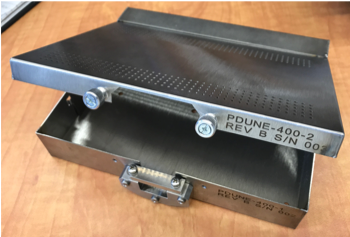
\includegraphics[width=0.45\linewidth]{sp-tpcelec-CEbox.png}
\end{dunefigure}

The \dword{ce} box casing is electrically connected to the \dword{apa} frame via the metal mounting hardware,
called the ``Omega bracket'' (not shown in Figure~\ref{fig:ce-box}), 
and the input amplifier circuits are connected to the CR board, which also terminate to
ground at the \dword{apa} frame, as shown in Figure~\ref{fig:CR-board}.
As a backup, the casing is also connected to the \dword{apa} frame via a twisted conducting wire.

In addition to the CE Box and mounting hardware, cable trays for support and routing the cold cables will be installed in the 
cryostat. One set of cable trays, shown in Figure~\ref{fig:upper-tray}, will be attached to the upper \dword{apa} itself 
to hold the CE and PD cables. A different cable tray design, shown in Figure~\ref{fig:lower-tray}, will be used
to support the CE and PD cables underneath the lower hanging APA. A final set of cable trays will be installed inside the 
cryostat after the APAs are fixed in their final location to support the cables as they are 
routed to the CE and PD feedthroughs.

\begin{dunefigure}
[Side and end views of mechanical supports for the \dword{ce} Boxes on the upper \dword{apa}. Shown are 
the APA cable trays in green, the CE Boxes in dark gray, and the Omega brackets between the CE Boxes 
and APA frame in light gray. Neither CE or PD cables are shown.]
{fig:upper-tray}
{Side and end views of mechanical supports for the \dword{ce} Boxes on the upper \dword{apa}. Shown are 
the APA cable trays in green, the CE Boxes in dark gray, and the Omega brackets between the CE Boxes 
and APA frame in light gray. Neither CE or PD cables are shown.}
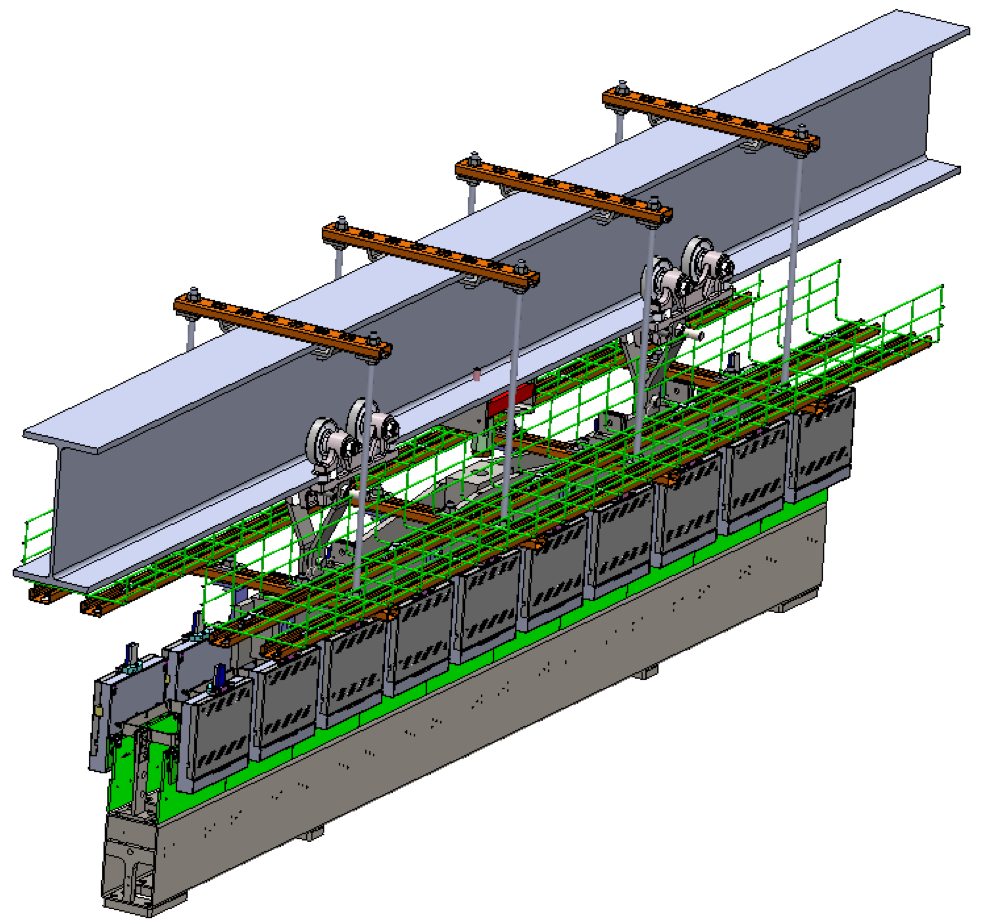
\includegraphics[width=0.4\linewidth]{sp-tpcelec-upper-tray1.png}
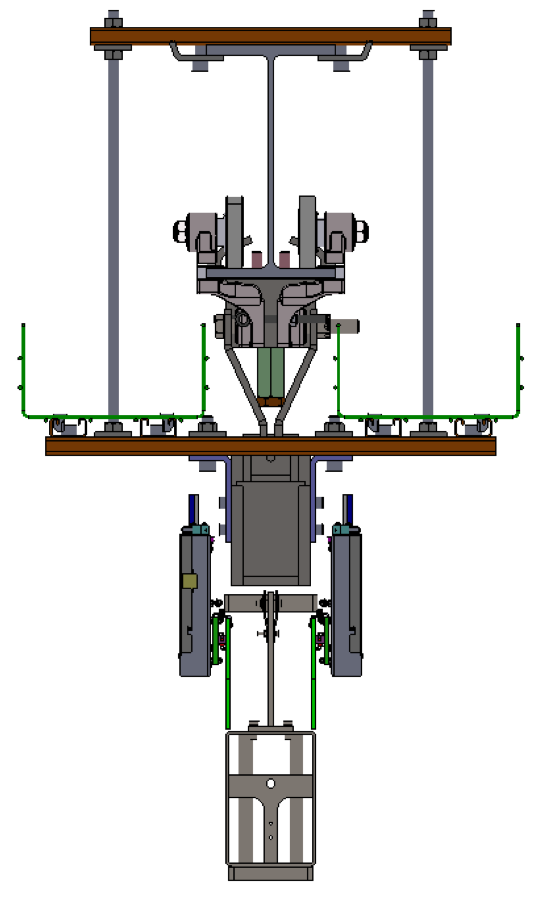
\includegraphics[width=0.4\linewidth]{sp-tpcelec-upper-tray2.png}
\end{dunefigure}

\begin{dunefigure}
[Side and end views of mechanical supports for the \dword{ce} Boxes on the lower \dword{apa}. Shown are 
the APA cable tray in pink, the CE Boxes in dark gray, and the Omega brackets and mounting hardware 
between the CE Boxes and APA frame in light gray. The CE cables are shown in blue; the PD cables are not shown.]
{fig:lower-tray}
{Side and end views of mechanical supports for the \dword{ce} Boxes on the lower \dword{apa}. Shown are 
the APA cable tray in pink, the CE Boxes in dark gray, and the Omega brackets and mounting hardware 
between the CE Boxes and APA frame in light gray. The CE cables are shown in blue; the PD cables are not shown.}
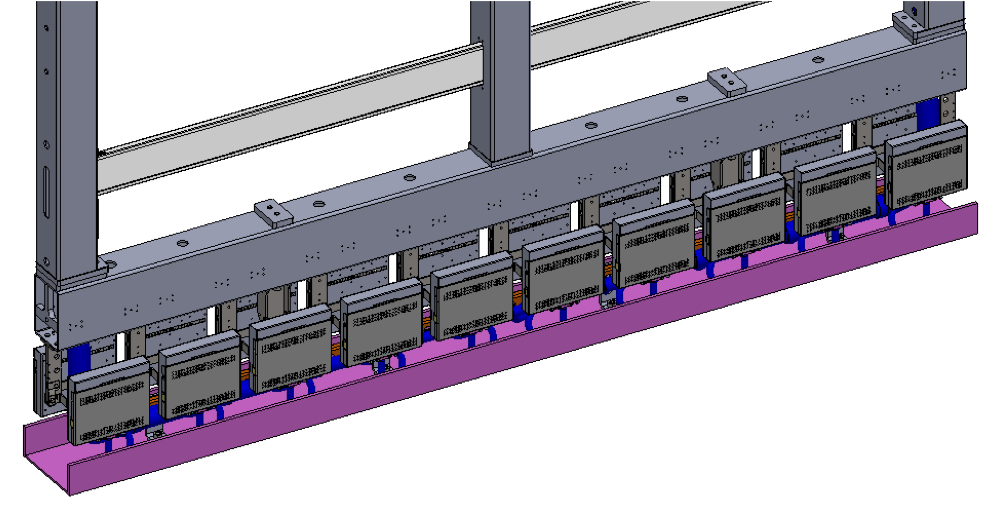
\includegraphics[width=0.4\linewidth]{sp-tpcelec-lower-tray1.png}
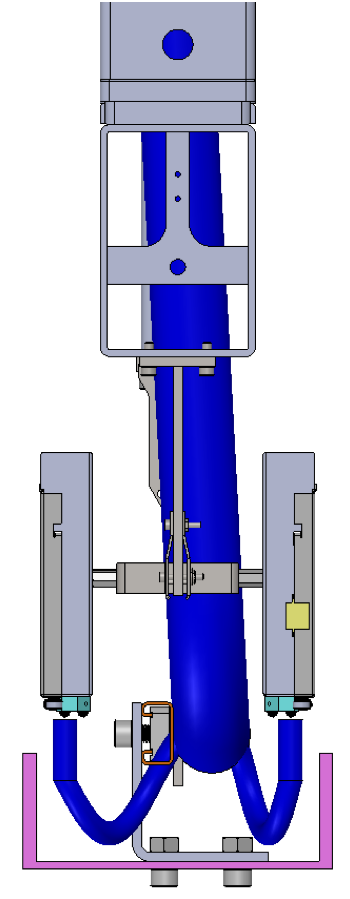
\includegraphics[width=0.4\linewidth]{sp-tpcelec-lower-tray2.png}
\end{dunefigure}

%%%%%%%%%%%%%%%%%%%%%%%%%%%%%%%%%%%
\subsection{Cold Electronics Feedthroughs}
\label{sec:fdsp-tpcelec-design-ft}

All cold cables originating from inside the cryostat connect to the outside warm electronics through PCB board \fdth{}s
installed in the signal flanges that are distributed along the cryostat roof.
The TPC data rate per \dword{apa}, with an overall \num{32}:\num{321} MUX and eighty $\sim$1~Gbps data channels per \dword{apa},
is sufficiently low that the \dword{lvds} signals can be driven over copper twin-axial transmission lines.
Additional transmission lines are available for the distribution of \dword{lvds} clock signals and I$^2$C control information,
which are transmitted at a lower bit rate.
Optical fiber is employed externally from the \dwords{wib} on the signal flange to the \dword{daq} and slow control systems described in Chapter~\ref{ch:fdsp-daq} and Chapter~\ref{ch:fdsp-slow-cryo}, respectively.

\begin{dunefigure}
[TPC \dword{ce} \fdth.]
{fig:tpcelec-signal-ft}
{TPC \dword{ce} \fdth. The \dwords{wib} are seen edge-on in the left panel, and in an oblique side-view in the right panel, which also shows the warm crate for a \dword{spmod} %DUNE module 
in a cutaway view.}
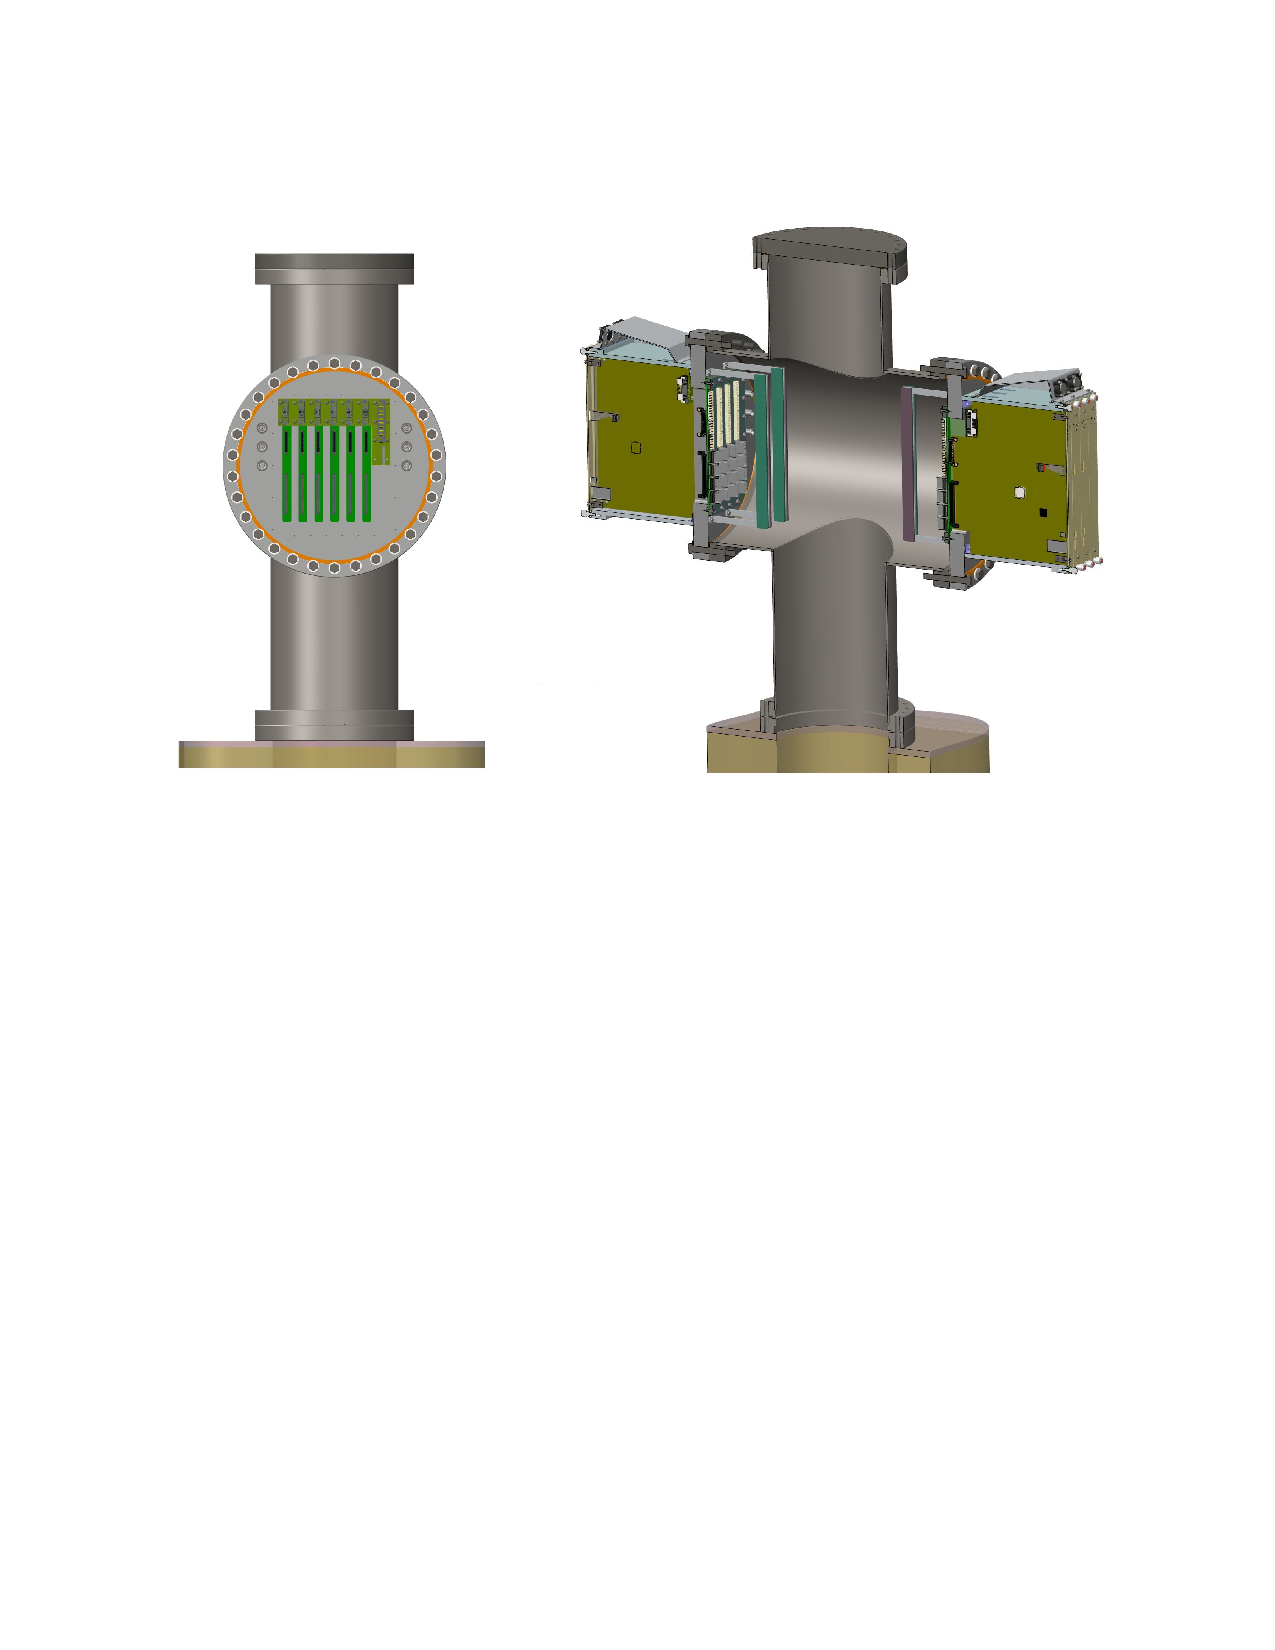
\includegraphics[width=0.9\linewidth]{sp-tpcelec-signal-FT.pdf}
\end{dunefigure}

The design of the signal flange includes a four-way cross spool piece, separate PCB \fdth{}s for the \dword{ce} and \dword{pds} cables, and
an attached crate for the TPC warm electronics, as shown in Figure~\ref{fig:tpcelec-signal-ft}.
The wire bias voltage cables connect to standard SHV (safe high voltage) connectors machined directly into the \dword{ce} \fdth,
ensuring no electrical connection between the wire bias voltages and other signals passing through the signal flange.
Each \dword{ce} \fdth serves the bias, power, and digital I/O needs of one \dword{apa}.  

Data and control cable bundles are used to send system clock and control signals from the 
signal flange to the \dword{femb}, stream the $\sim$\SI{1}{Gbps} high-speed data from the \dword{femb} to the signal flange.  Each \dword{femb} 
connects to a signal flange via one data cable bundle, leading to 20 bundles between one \dword{apa} and one flange.  Each data bundle contains 12 low-skew twin-axial cables with a drain wire, 
to transmit the following differential signals:
\begin{itemize}
    \item four \SI{1.28}{Gbps} data (two from each \dword{coldata});
    \item two \SI{64}{MHz} clocks (one input to each \dword{coldata});
    \item two fast command lines (one input to each \dword{coldata});
    \item three I$^2$C-like control lines (clock, data-in, and data-out); and
    \item one multipurpose \dword{larasic} output (temperature, reference voltage, or analog test output).
\end{itemize}

The \dword{lv} power is passed from the signal flange to the \dword{femb} by bundles of
20AWG twisted-pair wires. Half of the wires are power feeds; the others
are attached to the grounds of the input amplifier circuits, as described in Section~\ref{sec:fdsp-tpcelec-design-bias}.
For a single \dword{femb}, the resistance is measured to be  <\SI{30}{\milli\ohm} at room temperature or $<10$~m$\Omega$ at 
\lar temperature. Each \dword{apa} has a copper cross section of approximately %$80~\mathrm{mm}^2$ 
\SI{80}{mm$^2$}, with a 
resistance <\SI{1.5}{\milli\ohm} at room temperature or $<0.5$~m$\Omega$ at \lar temperature.

The bias voltages are applied to the $X$-, $U$-, and $G$-plane wire layers, three \dword{fc} terminations, 
and an electron diverter, as shown in Figure~\ref{fig:CR-board}. The voltages are supplied 
through eight SHV connectors mounted on the signal flange. RG-316 coaxial cables carry the voltages 
from the signal flange to a patch panel PCB which includes noise filtering mounted on the top 
end of the \dword{apa}. 

From there, wire bias voltages are carried by single wires to 
various points on the \dword{apa} frame, including the CR boards, a small PCB mounted on or near 
the patch panel that houses a noise filter and termination circuits for the field cage voltages, and 
a small mounted board near the electron diverter that also houses wire bias voltage filters.

%%%%%%%%%%%%%%%%%%%%%%%%%%%%%%%%%%%
\subsection{Warm Interface Electronics}
\label{sec:fdsp-tpcelec-design-warm}

The warm interface electronics provide an interface between the \dword{ce}, \dword{daq}, timing, and slow control systems, including local power control at the flange and a real-time diagnostic readout. They are housed in the \dwords{wiec} attached directly to the \dword{ce} flange.  The \dword{wiec} shown in Figure~\ref{fig:tpcelec-flange} contains one power and timing card (\dword{ptc}), five warm interface boards (\dwords{wib}) and a passive power and timing backplane (PTB), which fans out signals and \dword{lv} power from the \dword{ptc} to the \dwords{wib}. The \dword{wiec} must provide a Faraday-shielded housing, robust ground connections from the \dwords{wib} to the detector ground described in Section~\ref{sec:fdsp-tpcelec-design-grounding}, and only optical fiber links to the \dword{daq} and slow control in order to mitigate noise introduced at the \dword{ce} \fdth.

\begin{dunefigure}
[Exploded view of the \dword{ce} signal flange for \dword{pdsp}.]
{fig:tpcelec-flange}
{Exploded view of the \dword{ce} signal flange for \dword{pdsp}.  The design will be very similar for the \dword{spmod} \dword{ce} signal flange (with two \dword{ce} signal flanges per \fdth).}
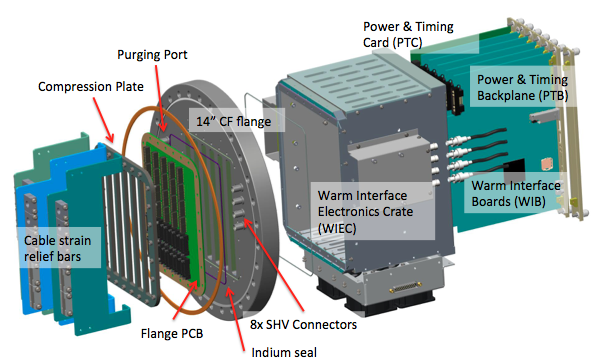
\includegraphics[width=0.9\linewidth]{sp-tpcelec-flange.png}
\end{dunefigure}

The \dword{wib} is the interface between the \dword{daq} system and four
\dwords{femb}. It receives the system clock and control signals from the
timing system and provides for processing and fan-out of those signals to the four
\dwords{femb}. The \dword{wib} also receives the high-speed data signals from the four 
\dwords{femb} and transmits them to the \dword{daq} system over optical
fibers. The data signals are recovered onboard the \dword{wib} with commercial equalizers.
The \dwords{wib} are attached directly to the TPC
\dword{ce} \fdth on the signal flange. The \fdth
board is a PCB with connectors to the cold signal and \dword{lv} power cables fitted
between the compression plate on the cold side, and sockets for
the \dword{wib} on the warm side. Cable strain relief for the cold cables is 
supported from the back end of the \fdth.

The \dword{pdsp} \dword{ptc} provides a bidirectional fiber interface to the
timing system. The clock and data
streams are separately fanned out to the five \dwords{wib} as shown in
Figure~\ref{fig:tpcelec-wib-timing}. The \dword{ptc} fans the clocks out to the \dword{wib} over the
PTB, which is a passive backplane attached directly to the \dword{ptc} and
\dwords{wib}.  The received clock on the \dword{wib} is separated into clock and
data using a clock-data separator. Timing endpoint firmware to receive and transmit
the clock is integrated in the \dword{wib} \dword{fpga} (the Altera Arria V\footnote{Altera Arria\texttrademark{}, V FPGA family, \url{https://www.altera.com/products/fpga/arria-series/arria-v/overview.html}.} was used for \dword{pdsp}).
The \dword{spmod} timing system, described in Section~\ref{sec:fd-daq-timing}, is a development of the \dword{pdsp} system, and expected to require the nearly identical functionality at the \dword{wib} endpoint.

\begin{dunefigure}
[\dword{pdsp} PTC and timing distribution to the WIB and FEMBs]
{fig:tpcelec-wib-timing}
{Power and timing card (\dword{ptc}) and timing distribution to the \dword{wib} and \dwords{femb} used in \dword{pdsp}.}
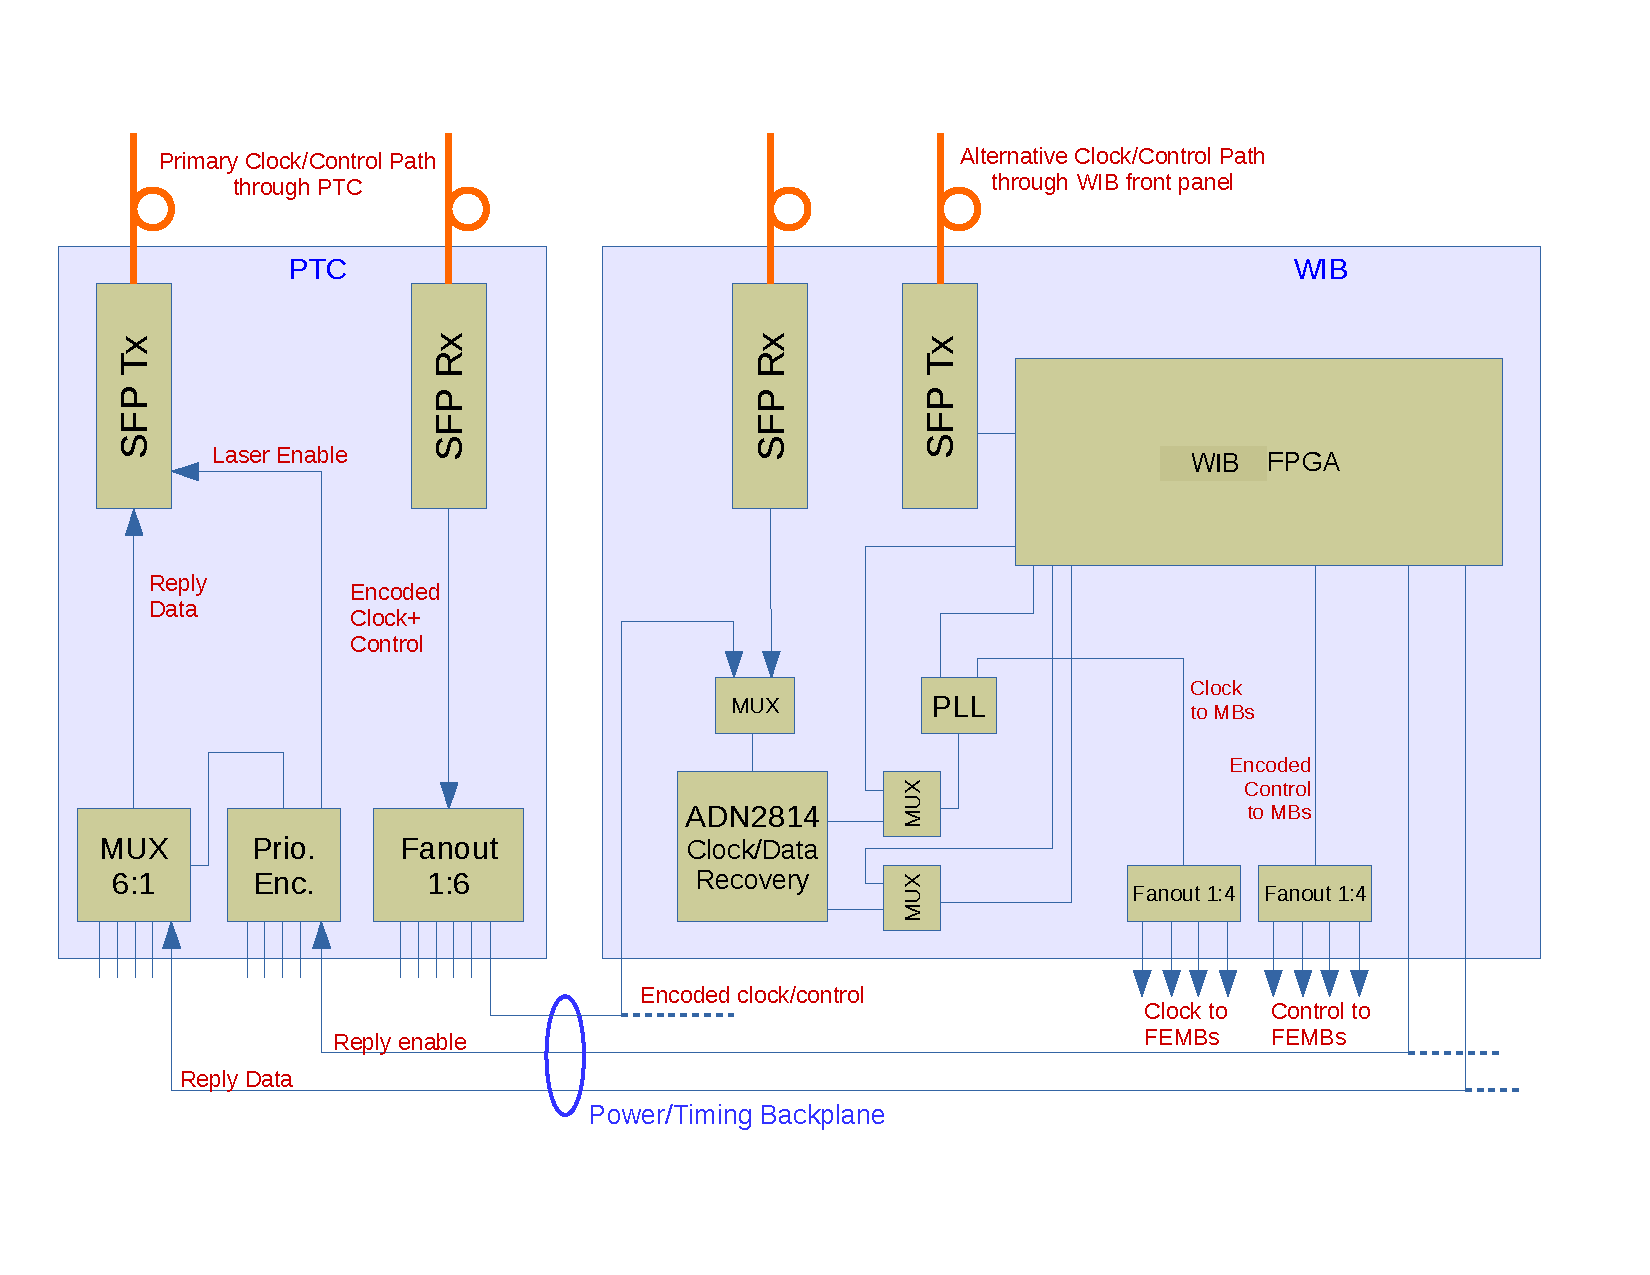
\includegraphics[width=0.75\linewidth]{sp-tpcelec-wib-timing-v2.pdf}
\end{dunefigure}

The \dword{ptc} also receives \SI{48}{V} \dword{lv} power for all cold
electronics connected through the TPC signal flange: one \dword{ptc}, five \dword{wib}, and \num{20}~\dword{femb}. The \dword{lv} power is then stepped down
to \SI{12}{V} via a DC-DC converter onboard the \dword{ptc}. The output of the \dword{ptc} converters is filtered with a common-mode choke and fanned out
on the PTB to each \dword{wib}, which provides the necessary \SI{12}{V} DC-DC conversions and fans
the \dword{lv} power out to each of the cold \dwords{femb} supplied by that \dword{wib}, 
as shown in Figure~\ref{fig:tpcelec-wib-power}. The output of the \dword{wib} converters is further filtered by a common-mode choke. The 
majority of the power drawn by a full flange is dissipated in the \lar by the cold \dword{femb}.

\begin{dunefigure}
[\dword{pdsp} \dword{lv} power distribution to the \dword{wib} and \dwords{femb}]
{fig:tpcelec-wib-power}
{\dword{lv} power distribution to the \dword{wib} and \dwords{femb} implemented for \dword{pdsp}. This will be modified for the \dword{spmod} to provide the required voltage or voltages depending on which \dwords{asic} are used on the \dwords{femb}. In particular the voltages to the \dword{femb} \numrange{0}{3} will change as the \dword{pdsp} \dword{fpga} is replaced by \dword{coldata}. }
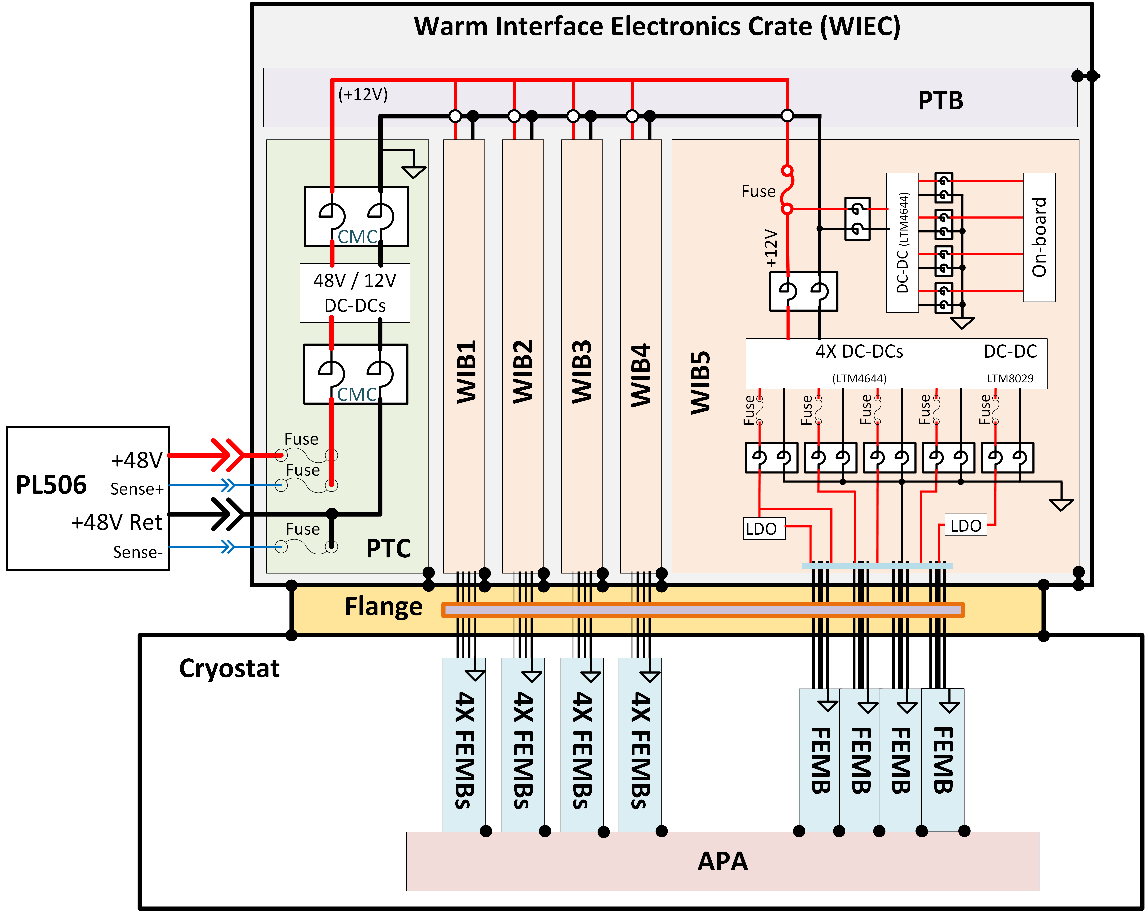
\includegraphics[width=0.65\linewidth]{sp-tpcelec-wib-power.pdf}
\end{dunefigure}

Because the \dwords{wib} can provide local power to the \dword{femb} and real-time diagnostic readout of all channels,
each CE system for each APA is a complete, stand-alone readout unit. The \dwords{femb} and cold cables are shielded
inside the cryostat and the \dwords{wib} and \dword{ptc} are shielded inside the Faraday cage of the warm interface
electronics crate, with only shielded power cables and optical fibers connecting to external systems.

As shown in Figure~\ref{fig:tpcelec-dune-wib}, the \dword{wib} is capable of receiving \dword{lv} power in the front panel and distributing it directly to the \dword{femb}, bypassing all DC/DC converters.
It can also receive the encoded system timing signals over bi-directional optical
fibers on the front panel, and process these using either
the on-board \dword{fpga} or clock synthesizer chip to provide the clock required by the \dword{ce}.
The baseline \dword{asic} design currently uses 8b/10b encoding; if the SLAC CRYO \dword{asic} is selected for
the DUNE \dword{spmod}, 12b/14b encoding will be used instead of 8b/10b.

\begin{dunefigure}
[Warm interface board (\dword{wib})]
{fig:tpcelec-dune-wib}
{Warm interface board (\dword{wib}). Note that front panel inputs include a LEMO connector and alternate inputs for \dword{lv} power and timing.}
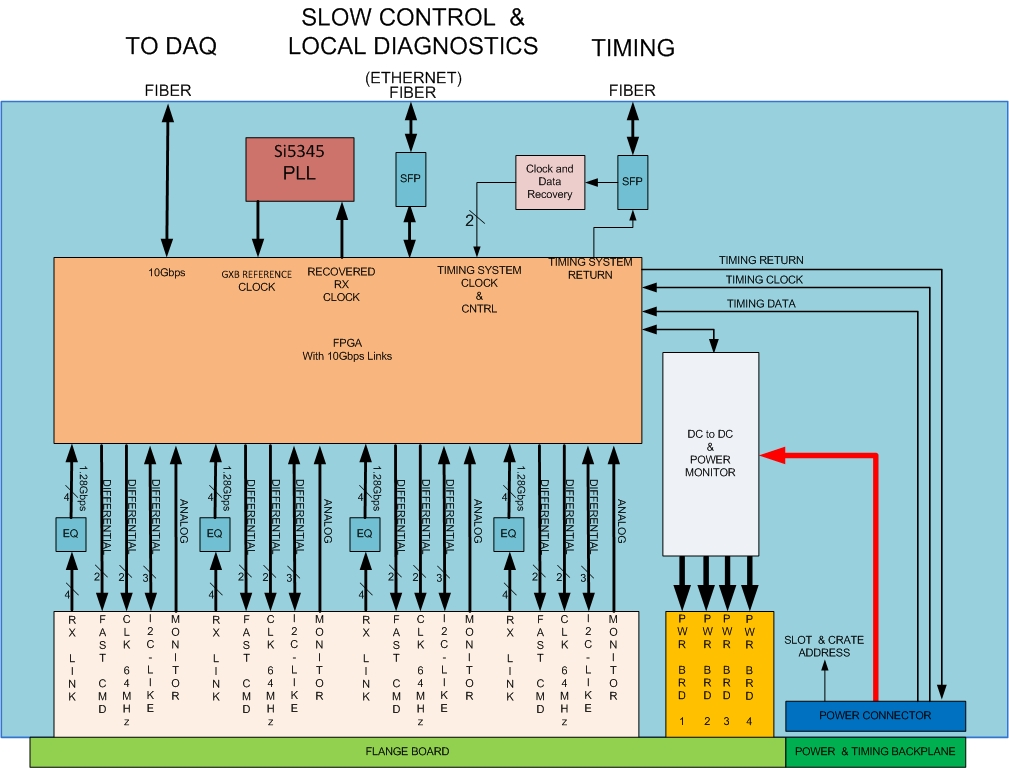
\includegraphics[width=0.8\linewidth]{sp-tpcelec-dune-wib.jpg}
\end{dunefigure}

The \dword{fpga} on the \dword{wib} will have
transceivers that can drive the high-speed data to the \dword{daq} system up to
10.3125~Gbps per link, implying that all data from
two \dword{femb} (2$\times$5~Gbps) could be transmitted on a single link.
The \dword{fpga} will have an additional Gbps Ethernet transceiver I/O based on the \SI{125}{MHz} clock, which 
provides real-time digital data readout to the slow control system.

%%%%%%%%%%%%%%%%%%%%%%%%%%%%%%%%%%%
\subsection{Services on Top of the Cryostat}
\label{sec:fdsp-tpcelec-design-services}

As implemented for \dword{pdsp}, a fully loaded \dword{wib} (one \dword{wib} plus four \dwords{femb}) requires
\SI{12}{V} and draws up to approximately \SI{4}{A}. The full electronics for one \dword{apa} (one \dword{ptc}, five \dwords{wib}, and \num{20} \dwords{femb}) 
requires \SI{12}{V} and draws approximately \SI{20}{A}, for a total power of approximately \SI{240}{W}, as 
described in Section~\ref{sec:fdsp-tpcelec-design-warm}. The \dword{spmod} implementation should require much 
less power as the \dword{fpga} will be replaced by the \dword{coldata} chips.

As the \dword{lv} power is delivered at \SI{48}{V} to the \dword{ptc}, each \dword{lv} power mainframe is chosen to bracket that value; each has  
roughly \numrange{30}{60}{V}, \SI{13.5}{A}, \SI{650}{W} maximum capacity per \dword{apa}. Using 10AWG cable, a \SI{0.8}{V} drop is 
expected along the cable with a required power of \SI{306}{W} out of \SI{650}{W} available.  
This leaves a significant margin that allows for larger distances between the power supplies and 
the warm interface crates than the \SI{20}{\meter} in \dword{pdsp}.

Four wires are used for each module; two 10AWG, shielded, twisted-pair cables for the power and return; and two 20AWG, shielded, twisted-pair cables for the sense.
The primary protection is the over-current protection circuit in the \dword{lv} supply modules, 
which is set above the \SI{20}{A} current draw of the \dword{wiec}.  Secondary sense line fusing is 
provided on the \dword{ptc}.  The \dword{lv} power cable uses FCi micro TCA\footnote{MicroTCA\texttrademark{} (\dword{utca}) vertical card-edge connectors, Amphenol ICC,  \url{https://www.amphenol-icc.com/product-series/micro-tca-card-edge.html}.} connectors, shown in
Figure~\ref{fig:tpcelec-powerconn}.

% we can think about removing this figure
\begin{dunefigure}
[FCi microTCA power connector at the \dword{ptc} end of the cable.]
{fig:tpcelec-powerconn}
{FCi microTCA power connector at the \dword{ptc} end of the cable.}
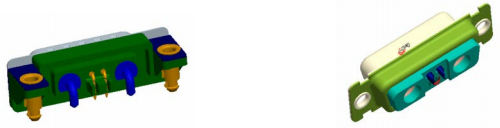
\includegraphics[width=0.9\linewidth]{sp-tpcelec-power-connector.png}
\end{dunefigure}

An 18V linear power supply will provide power to the cooling fans for the WIEC. It will be interlocked to the 48V power 
supplies, so the WIBs may not be powered without the cooling fans in operation. A 10V power supply will provide
power to the 4 heating elements on each PD and CE flange.

Bias voltages for the \dword{apa} wire planes, the electron diverters, and the last \dword{fc} electrodes are generated 
by supplies which are the responsibility of the TPC Electronics consortium.  The current from each of these supplies 
is expected to be very close to zero in normal operation.  However, the ripple voltage must be carefully controlled to 
avoid injecting noise into the front-end electronics.  RG-58 coaxial cables connect the wire bias voltages from the 
mini-crate to the standard SHV connectors machined directly into the \dword{ce} \fdth, so there is no electrical 
connection between the \dword{lv} power and data connectors and wire bias voltages.

Optical fibers are used for all connections between the \dwords{wiec}, which act as
Faraday-shielded boxes, and the \dword{daq} and slow control systems.  The \dword{wib} reports
its onboard temperature and the current draw from each \dword{femb} to the slow control system, while the
current draw for each \dword{apa} is monitored at the mainframe itself.

To support the electronics, fan, and heater power cables and optical fibers on top of the cryostat, 
cable trays will be installed. Racks for all the necessary \dword{lv} supplies will be installed on a mezzanine
near the cryostat roof, as shown in Figure~\ref{fig:cryostat-roof}.
Additionally, patch panels will be installed on top of the cryostat to separate the data and timing optical fibers and gigE
cables going to the PTC and WIBs from the long cable run to the DAQ.

\begin{dunefigure}
[Services on top of the cryostat. The racks for the \dword{lv} power supplies are shown in blue.]
{fig:cryostat-roof}
{Services on top of the cryostat. The racks for the \dword{lv} power supplies are shown in blue.}
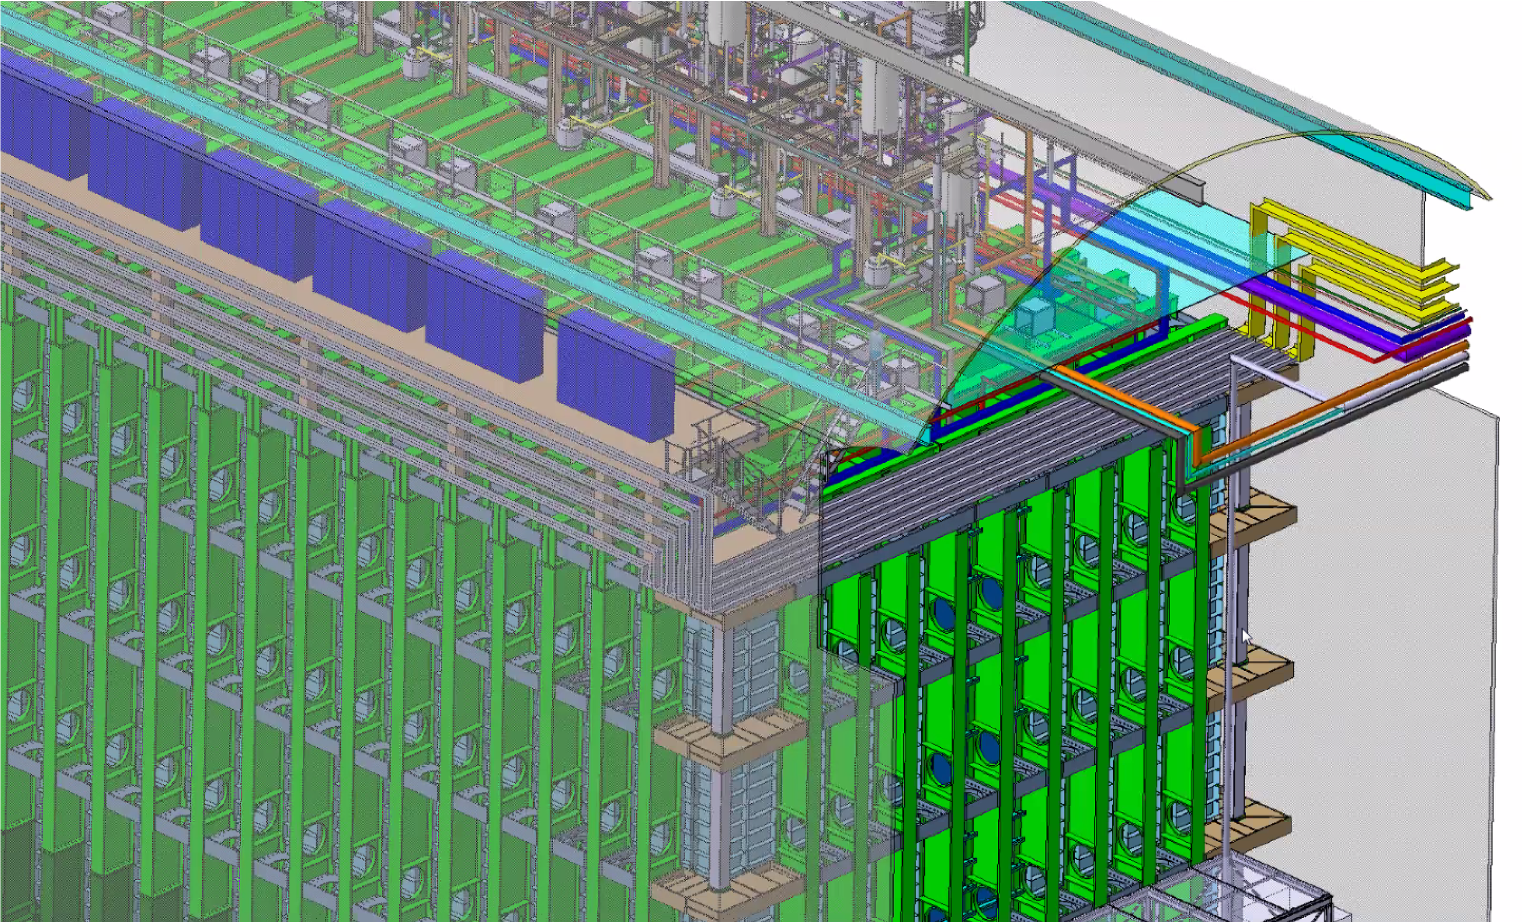
\includegraphics[width=0.9\linewidth]{sp-tpcelec-cryostat-top.png}
\end{dunefigure}
